%%%%%%%%%%%%%%%%%%%%%%%%%%%%%%%%%%%%%%%%%%%%%%%%%%%%%%%%%%%%%%%%%%%%%%%%
% 
% LaTeX Template
%
%%%%%%%%%%%%%%%%%%%%%%%%%%%%%%%%%%%%%%%%%%%%%%%%%%%%%%%%%%%%%%%%%%%%%%%%

%------------------------------------------------------------------------------------------------
%	DOCUMENT CONFIGURATIONS
%------------------------------------------------------------------------------------------------

% DOCUMENT
%   - Properties
\documentclass[a4paper,11pt]{report} % Sets a two-sided A4 sized paper.
                                         % (Two-sided for LaTeX to distinguish between odd/even
                                         % pages while using headers and footers.)
\linespread{1.15}                         % Default space between lines
                                    % Margin sizes defined in headers_and_footers file.
\usepackage[nottoc,numbib]{tocbibind}    % Makes References section appear in the Table of contents (nottoc). Conuts the References like section.
\usepackage{lastpage}                    % To get the total number of pages.

%   - Sectioning
\usepackage{titlesec}                   % Extra features for sectioning
    % The following lines create: \subsubsubsection{}
    
    
%%%%%%%%% From here: creation of \subsubsubsection{} %%%%%%%%%
    \titleclass{\subsubsubsection}{straight}[\subsection]

    \newcounter{subsubsubsection}[subsubsection]
    \renewcommand\thesubsubsubsection{\thesubsubsection.\arabic{subsubsubsection}}
    \renewcommand\theparagraph{\thesubsubsubsection.\arabic{paragraph}} % optional; useful if paragraphs are to be numbered

    \titleformat{\subsubsubsection}
      {\normalfont\normalsize\bfseries}{\thesubsubsubsection}{1em}{}
    \titlespacing*{\subsubsubsection}
    {0pt}{3.25ex plus 1ex minus .2ex}{1.5ex plus .2ex}

    \makeatletter
    \renewcommand\paragraph{\@startsection{paragraph}{5}{\z@}%
      {3.25ex \@plus1ex \@minus.2ex}%
      {-1em}%
      {\normalfont\normalsize\bfseries}}
    \renewcommand\subparagraph{\@startsection{subparagraph}{6}{\parindent}%
      {3.25ex \@plus1ex \@minus .2ex}%
      {-1em}%
      {\normalfont\normalsize\bfseries}}
    \def\toclevel@subsubsubsection{4}
    \def\toclevel@paragraph{5}
    \def\toclevel@paragraph{6}
    \def\l@subsubsubsection{\@dottedtocline{4}{7em}{4em}}
    \def\l@paragraph{\@dottedtocline{5}{10em}{5em}}
    \def\l@subparagraph{\@dottedtocline{6}{14em}{6em}}
    \makeatother

    \setcounter{secnumdepth}{4}
    \setcounter{tocdepth}{4}
%%%%%%%%% Until here: creation of \subsubsubsection{} %%%%%%%%%


%\let\oldsection\section % This line and the following force sections to start on odd pages.
%\def\section{\cleardoublepage\oldsection}

\newcommand*{\blankpage}{%
    \vspace*{\fill}
        \begin{center}
            (This page was intentionally left in blank.)
        \end{center}
    \vspace{\fill}
}
\makeatletter
\renewcommand*{\cleardoublepage}{\clearpage\if@twoside \ifodd\c@page\else
\blankpage
\thispagestyle{empty}
\newpage
\if@twocolumn\hbox{}\newpage\fi\fi\fi}
\makeatother

% WRITING
%   - Math/Chemistry/...
\usepackage{amsmath}                % Mathematical features.
    % Section numbering
    \numberwithin{equation}{section}    % Equation numbering by section
    \numberwithin{table}{section}       % Table numbering by section
    \numberwithin{figure}{section}      % Table numbering by section
\usepackage{amssymb}                % Symbols.
\usepackage[version=3]{mhchem}                 % Chemical equation typesetting. i.e.: \ce{CO2 + C <=> 2CO}
\usepackage{siunitx}                % Simplifies the usage of values with units.
                                    % i.e.: "\SI{5.4}{kg·m^{-1}·s^{-2}}"
                                    % instead of "5.4 kg·m$ ^{-1} $·s$ ^{-2} $"
\usepackage{eurosym}                % Use EURO symbol (\euro)

%%   - Language
\usepackage[utf8]{inputenc}         % Required for the usage of characters like 'ñ', 'ú', ...
%\renewcommand{\figurename}{Figura}  % In captions, print "Figura" (in Catalan) instead of
                                    % "Figure" (English default name).
%\renewcommand{\tablename}{Tabla}
%\renewcommand{\contentsname}{Índice}
%\renewcommand{\refname}{Bibliografía}

%   - Text
%\let\oldsection\section             % This line and the nextone force sections to start always in new odd pages.
%\def\section{\cleardoublepage\oldsection} %
\usepackage[none]{hyphenat}         % [none] Prevents any hyphenation throughout the document.
                                    % (hyphenation -> "separació per síl·labes")
\sloppy                             % Forces wrapping at word boundaries by relaxing the interword space constraints.
%\usepackage{indentfirst}            % Forces indentation from paragraphs after a section.
                                    % (see notes 1 and 2)
\setlength\parindent{1cm}           % Removes all indentation from paragraphs.
%\newenvironment{paragraphs}{\setlength\parindent{1cm}}{\setlength\parindent{0cm}}
                                    % "\begin{paragraphs}" will create an environment where
                                    % indentation from paragraphs is activated.
\usepackage[font=footnotesize]{caption} % Captions
\setlength{\abovecaptionskip}{0pt}      %
\setlength{\belowcaptionskip}{0pt}      %
\usepackage{lmodern}                % Allow the use of font size larger tha 25pt
\usepackage[T1]{fontenc}            %

% GRAPHICS, TABLES AND OTHERS
\usepackage{graphicx}               % Required for the inclusion of images.
\usepackage{float}                  % Required for some float properties.
\usepackage{pdfpages}               % Required for the inclusion of PDF files.
\usepackage{multirow,longtable,array,booktabs,tabularx} % More features for tables.
\usepackage{enumerate}              % Gives the enumerate environment an optional argument which
                                    % determines the style in which the counter is printed.
\usepackage{enumitem}               % Extra options for "enumerate" lists
\usepackage{color}                  % Use some color options.
\usepackage{colortbl}               % Use some other color options.
	\definecolor{UPC_blue}{RGB}{67,142,197}
	\definecolor{lightgrey}{RGB}{166,166,166}
\usepackage{hyperref}               % Provides LeTeX the hability to create hyperlinks.

\usepackage{inputenc}         % It makes possible to use roman numbers for the pages before the first chapter and arabic for the rest of the document

\usepackage{booktabs}
\usepackage{xcolor,colortbl}
\usepackage{pstricks}
\usepackage{blindtext}
\usepackage{transparent}
\usepackage{etoolbox}
\usepackage{pdflscape}
\usepackage{amsmath}
\usepackage{amsfonts}
\usepackage{amssymb}
\usepackage{graphicx}
\usepackage{eurosym}
\usepackage{wrapfig}
\usepackage{mathdots}
\usepackage{caption}
\usepackage{cite}
\usepackage{mathrsfs}
\usepackage{float}
\usepackage{import}
\usepackage{makecell}
\usepackage{booktabs}
\usepackage{graphicx}

%   - NOTES
% (1) LaTeX implements a style that doesn't indent the first paragraph after a section heading. There are coherent reasons for this. Some typography rules state that first indent should be suppressed only after a centered title and that all other paragraphs must be indented.
% (2) We have already removed all indentation from paragraphs with the command "\setlength\parindent{0cm}", but when using the environment we've created "escrit" we set indent to 1cm. Then, if this environment is used right after a section the first indent will be suppressed unless we use the package "indentfirst". % Document Configurations

%-----------------------------------------------------------------------------
%	REPORT INFORMATION
%-----------------------------------------------------------------------------

%%% MAIN INFORMATION %%%

% School
\newcommand{\School}{ESEIAAT}
\newcommand{\researcherDept}{UPC - HIRO}
% Degree
\newcommand{\Degree}{Aerospace Technology Engineering}

% Department
\newcommand{\Department}{UPC Departament d'Enginyeria de Projectes i de la Construcció}

% Secció (Secció de Terrassa)
\newcommand{\Seccio}{Secció de Terrassa}

% Course
\newcommand{\Course}{Degree Final Project}

% Group
\newcommand{\Group}{G3-PM-P2018}

% Students (if you don't use that much students, leave them in blank)
\newcommand{\Studi}	    {Calderón Rosario, Borja}
\newcommand{\Studii}	{De Benedicto Barba, Maria}
\newcommand{\Studiii}	{Escartín Vivancos, Guillermo}
\newcommand{\Studiv}	{Fontanes Molina, Pol}
\newcommand{\Studv}	    {Franch I Ruiz, Sergi}
\newcommand{\Studvi}	{González García, Sílvia}
\newcommand{\Studvii}	{Herrando Moraira, Albert}
\newcommand{\Studviii}	{Lopezbarrena Arenas, Santiago}
\newcommand{\Studix}	{Nachett, Hamza}
\newcommand{\Studx}	    {Pérez Sánchez, David}
\newcommand{\Studxi}	{Pla Olea, Laura}
\newcommand{\Studxii}	{Pons Daza, Marina}
\newcommand{\Studxiii}	{Ramón Costa, Fernando}
\newcommand{\Studxiv}	{Sellart Combalia, Ana Maria}
\newcommand{\Studxv}	{Serra Moncunill, Josep Maria}
\newcommand{\Studxvi}	{Urbano González, Eva María}


% Customer:
\newcommand{\Director}{Pérez Llera, Luís Manuel}
\newcommand{\CoDirector}{Williams, Earle}

% Project Name
\newcommand{\ProjectName}{Project DEOS-UD}
\newcommand{\ProjectsubName}{Disruptive Earth Observation Sensing for Urban Developement}
% Acronym
\newcommand{\Acronym}{HIRO}

% Short Name
\newcommand{\ShortName}{HIRO}

% Kind of document
\newcommand{\DocTypeI}{Deliverable 1}
\newcommand{\DocTypeII}{Project Charter}

% Page number preceding (leave in blank if nothing is required)
% Suggestion: R, RA, B, D, T referred to report, report attachments, budget, drawings or technical sheets
\newcommand{\precPage}{PC}


% Date of the document (Delivery date)
	% Day
	\newcommand{\DocDateD}{16}
	% Month
	\newcommand{\DocDateM}{03}
	% Year
	\newcommand{\DocDateY}{2018}

%-----------------------------------------------------------------------------
% Don't touch this unless you know what you are doing!

% Generation of Group Code
\newcommand{\GrCode}{{\GrNum} EA-\GrTerm\GrYr} 

% Generation of the date format
\newcommand{\DocDate}{\DocDateD-\DocDateM-\DocDateY}  % Document information

%-----------------------------------------------------------------------------
%	HEADERS AND FOOTERS
%-----------------------------------------------------------------------------

% Changes default margins.
\usepackage[left=3cm,right=3cm,top=2.5cm,bottom=2.5cm]{geometry}
   \setlength{\headheight}{50pt}         % Header Space.
   \setlength{\textheight}{640pt}        % Text height.
   \setlength{\footskip}{30pt}           % Foot Space.

\usepackage{fancyhdr}
	\pagestyle{fancy} % Headers and footers -> "fancy" style.
	
	% Obtain the name of the section:
	\renewcommand{\sectionmark}[1]{\markright{Section \thesection : #1}}
	\renewcommand{\chaptermark}[1]{\markleft{Chapter \thechapter : #1}} 

	\fancyhf{} % Clear all headers and footers fields

% Package info and examples
%		% O/E = Odd/Even page // L/C/R = Left/Center/Right field
%	\fancyhead[LE]{\hspace{-10pt}
%		\raisebox{-\height+12pt}{
%		
\includegraphics[height=30pt]{./doc_config/images/UPC_dpt}
%		}
%	}
%	\fancyhead[RE]{\bf \Department}
%	\fancyhead[LO]{\bf \DocType}
%	\fancyhead[RO]{\bf \emph{\ProjectName}}
%	\fancyfoot[LE,RO]{\thepage} % Adds customized pages numbers



%-----------------------------------------------
% General headers and footers of the document:
%-----------------------------------------------
	% Headers
	\fancyhead[LO]{\textbf{\rightmark}} % Section mark
	\fancyhead[RO]{
\includegraphics[height=25pt]{./doc_config/images/logo3}}
	\fancyhead[LE]{\textbf{\rightmark}}
	\fancyhead[RE]{
\includegraphics[height=25pt]{./doc_config/images/logo3}}

	% Footers
	\fancyfoot[CE,CO]{\precPage{} - \thepage}
	\fancyfoot[LO,RE]{\textbf{\Acronym}}

	\renewcommand{\headrulewidth}{0.5pt} % Header decorative line
	\renewcommand{\footrulewidth}{0.5pt} % Footer decorative line
	\renewcommand{\chaptermark}[1]{%
\markboth{#1}{}}
\renewcommand{\sectionmark}[1]{\markright{#1}}


%-----------------------------------------------
% Headers and footers for pages where chapter starts:
%-----------------------------------------------
\fancypagestyle{plain}{
	%Headers
	\fancyhead[LO]{\textbf{\leftmark}} % Section mark
	\fancyhead[RO]{
\includegraphics[height=25pt]{./doc_config/images/logo3}}
	\fancyhead[LE]{\textbf{\leftmark}}
	\fancyhead[RE]{
\includegraphics[height=25pt]{./doc_config/images/logo3}}
	%Footers
	\fancyfoot[CE]{\precPage{} - \thepage}
	\fancyfoot[CO]{\precPage{} - \thepage}
	\fancyfoot[LO,RE]{\textbf{\Acronym}}
	
	\renewcommand{\headrulewidth}{0.5pt} % Header decorative line
	\renewcommand{\footrulewidth}{0.5pt} % Footer decorative line
}


%-----------------------------------------------
% Cover headers and footers:
%-----------------------------------------------

	\fancypagestyle{CoverPage}{ % This creates a new headers and footers page style.
	                            % To use it type "\thispagestyle{FirstPage}" on the first page.
	                                % (right after "\maketitle")
		\fancyhf{}
		%\fancyfoot[C]{Group \GrCode \hfill [\DocDate]}
		\renewcommand{\headrulewidth}{0pt}
		\renewcommand{\footrulewidth}{0pt}
	}


%-----------------------------------------------
% No headers nor footers page (ie: Back cover)
%-----------------------------------------------

	\fancypagestyle{EmptyPage}{
		\fancyhf{}
		\renewcommand{\headrulewidth}{0pt}
		\renewcommand{\footrulewidth}{0pt}
	} % Headers and footers

%-----------------------------------------------------------------------------
%	USER DEFINED ENVIRONMENTS
%-----------------------------------------------------------------------------

% Itemize with reduced vertyical space between items
\newenvironment{itemize_rvs}
{ \begin{itemize}
    \setlength{\itemsep}{0pt}
    \setlength{\parskip}{0pt}
    \setlength{\parsep}{0pt}     }
{ \end{itemize}                  }

% Standard names

% Titles and sections structures
\newcommand{\subpart}[1]{\mbox{ }\\\noindent\textbf{#1}}
\newcommand{\subsubpart}[1]{\mbox{ }\\\indent\underline{#1}}
\newcommand{\subsubsubpart}[1]{\mbox{ }\\\indent\indent\textit{#1}}

% Figure/table source
\newcommand{\source}[1]{\caption*{\hfill Source: {#1}} } % User defined environments

% Paragraph formatting
\setlength{\parindent}{0pt}

\usepackage{epigraph}
\usepackage{tocloft}
\usepackage{multicol}
\usepackage[T1]{fontenc}
\usepackage{titlesec, blindtext, color}
\definecolor{gray75}{gray}{0.75}
\newcommand{\hsp}{\hspace{20pt}}
\titleformat{\chapter}[hang]{\Huge\bfseries}{\thechapter\hsp\textcolor{gray75}{|}\hsp}{0pt}{\Huge\bfseries}

\renewcommand{\familydefault}{\sfdefault}

\begin{document}

%-----------------------------------------------------------------------------
%	Project Charter Cover
%-----------------------------------------------------------------------------

\thispagestyle{CoverPage}

% Centered cover page

\begin{center}\bf

\begin{figure}[!tbp]
  \centering
  \begin{minipage}[b]{0.4\textwidth}
    \centering
      
\includegraphics[width=0.55\textwidth]{./doc_config/images/logo.png}
  \end{minipage}
  \hfill
  \begin{minipage}[b]{0.5\textwidth}
    \centering
         \raisebox {0.5cm} {
\includegraphics[width=0.9\textwidth]{./doc_config/images/UPC_dpt} }
  \end{minipage}
\end{figure}

% 
\includegraphics[width=0.2\textwidth]{./doc_config/images/logo2.png}\\
% \large \researcherDept

% \vspace{35pt}

% 
\includegraphics[width=0.4\textwidth]{./doc_config/images/UPC_dpt}\\
% {\large \School}

\vspace{5cm}

\begin{figure}[!tbp]
    \centering
         
\includegraphics[width=0.35\textwidth]{./doc_config/images/logo2.png}
\end{figure}

\vspace{2cm}

%{\Huge \ProjectName}\\
{\fontsize{25pt}{20pt}\selectfont \ProjectName}\\ \vspace{0.3cm}
{\fontsize{22pt}{20pt}\selectfont \ProjectsubName}


\vspace{10pt}

% {\fontsize{18pt}{20pt}\selectfont \Acronym}

%\includegraphics[width=0.4\textwidth]{./doc_config/images/DF_logo}

\textcolor{UPC_blue}{\rule{\textwidth}{.6pt}}

{\Large \DocTypeI}\\
{\Large \DocTypeII}

\end{center}

\vspace{20pt}

\textbf{Authors:}\vspace{7pt}

\begin{tabular}{ll}
	\Studi    \hspace*{30pt} & \Studix   \\
	\Studii   \hspace*{30pt} & \Studx   \\
	\Studiii  \hspace*{30pt} & \Studxi   \\
	\Studiv   \hspace*{30pt} & \Studxii \\
	\Studv    \hspace*{30pt} & \Studxiii    \\
	\Studvi   \hspace*{30pt} & \Studxiv  \\
	\Studvii  \hspace*{30pt} & \Studxv  \\
	\Studviii \hspace*{30pt} & \Studxvi  \\
\end{tabular}\\

\vspace{10pt}
\textbf{National Contact Point:} \Director\\

\vspace{10pt}
\textbf{Group:} \Group \hspace*{160pt} \textbf{Delivery date:} \DocDate
 % COVER
\newpage\thispagestyle{EmptyPage}
\mbox{}\newpage

\pagenumbering{roman}

% TABLE OF CONTENTS
\setcounter{tocdepth}{3}
\tableofcontents
\pagebreak

%\mbox{}\newpage
\renewcommand{\cfttabnumwidth}{4em}
\listoftables
\pagebreak

%\mbox{}\newpage
\renewcommand{\cftfignumwidth}{4em}
\listoffigures


% DOCUMENT SECTIONS

\newpage
\pagenumbering{arabic}

\newpage
\setlength{\parskip}{1em}



\chapter{Esto es un capítulo numerado}

Se genera con \verb!\chapter{Texto}!

\chapter*{Esto es un capítulo sin numerar}

Se genera con \verb!\chapter*{Texto}!

En este caso la numeración no sigue (es decir, que si el anterior capítulo numerado era el 1, este no cuenta, y el siguiente capítulo numerado será el 2). Tampoco aparece en la tabla de contenidos.

\chapter{Nuevo capítulo}

\section{Esto es una sección numerada}

Se genera con \verb!\section{Texto}!

\section*{Esto es una sección sin numerar}

Se genera con \verb!\section*{Texto}!

Aquí tampoco sigue la numeración ni aparece en la tabla de contenidos. Lo mismo se aplica a niveles inferiores

\section{Nueva sección}

\subsection{Esto es una subsección numerada}

Se genera con \verb!\subsection{Texto}!

\subsection*{Esto es una subsección sin numerar}

Se genera con \verb!\subsection*{Texto}!

\subsection{Nueva subsección}

\subsubsection{Esto es una subsubsección numerada}

Se genera con \verb!\subsubsection{Texto}!

\subsubsection*{Esto es una subsubsección sin numerar}

Se genera con \verb!\subsubsection*{Texto}!

\subsubsection{Nueva subsubsección}

\subsubsubsection{Esto es una subsubsubsección numerada}

Se genera con \verb!\subsubsubsection{Texto}!

\subsubsubsection*{Esto es una subsubsubsección sin numerar}

Se genera con \verb!\subsubsubsection*{Texto}!

\subsubsubsection{Nueva subsubsubsección}
\chapter{Párrafos}

Un párrafo se puede empezar a escribir tal cual, sin poner comandos ni ostias. Y cuando se quiere terminar el párrafo, se le da a enter dos veces, para que quede un espacio blanco en los dos cuerpos de texto del LaTex.

Y se sigue uno nuevo debajo.
Si solo se da un enter y se escribe justo debajo ocurre esto:
Que lo pilla todo como un mismo párrafo (como es el caso).

Un modo de escribir líneas una debajo de otra \newline
Es con el comando \verb!\newline! \newline
Alternativamente, se puede usar \verb!\\! \\
Y funciona de la misma forma

\paragraph{}Otro modo de empezar un párrafo es escribiendo el comando \verb!\paragraph{}!, que en este caso genera un párrafo con sangría (la primera del párrafo empieza un poco más adelante que el resto de líneas).

\paragraph{Título del párrafo}Si se rellenan los \verb!{}! del comando, como en \verb!\paragraph{Título del párrafo}!, el párrafo pasa a tener un título delante. En este caso, el párrafo no tiene sangría.

Destacar que si se crea un párrafo con \verb!\paragraph{}! (con o sin título), éste deja una distancia más grande con el texto anterior que si simplemente se le da a enter (comparar este párrafo con enter, como en anterior con el comando)
\chapter{Formato del texto}

Las opciones más importantes para dar formato al texto ya vienen, tanto en TeXmaker como en TeXstudio, en una columna a la izquierda del editor de texto (en la parte donde escribes, pues justo a la izquierda, es la columna que tiene una B, I, U arriba). Se puede hacer clic en la opción y luego introducir el texto, o seleccionar el texto y hacer clic.

\textbf{Texto en negrita}. Se crea con \verb!\textbf{Texto en negrita}!

\textit{Texto en cursiva}. Se crea con \verb!\textit{Texto en cursiva}!

\underline{Texto subrayado}. Se crea con \verb!\underline{Texto subrayado}!

Texto justificado para que ocupe todo el ancho de la hoja, siempre-y-cuando-no-sea-el-final-del-párrafo. Por defecto todos los textos se justifican automáticamente, de modo que no hay que preocuparse.

\begin{flushleft}
	Texto ajustado a la izquierda, de modo que aunque cuando se cambia de línea, no se ensancha la línea para que ocupe todo el ancho de la hoja, y da lugar a un borde derecho irregular. \newline
	Para esto se pone el comando \verb!\begin{flushleft}! \newline
	A continuación se escribe texto. \newline
	Y se cierra con \verb!\end{flushleft}!
\end{flushleft}

\begin{flushright}
	Texto ajustado a la derecha. \\
	Para esto se pone el comando \verb!\begin{flushright}! \\
	A continuación se escribe texto. \\
	Y se cierra con \verb!\end{flushright}! \\
	Para estos casos, si se quiere empezar una línea justo debajo, mejor con \verb!\\!
\end{flushright}

\begin{center}
	Texto centrado.\\
	Para esto se pone el comando \verb!\begin{center}! \\
	A continuación se escribe texto. \\
	Y se cierra con \verb!\end{center}!
\end{center}

Si se quiere generar un espacio vacío \hspace{1cm} tanto delante como en medio de un párrafo, se puede usar \verb!\hspace{1cm}!, que en este caso genera un espacio vacío de 1cm

A continuación vienen ejemplos de texto a distintos tamaños de letra. 

{\tiny Texto. Se hace con \verb!{\tiny Texto}!}

{\scriptsize Texto. Se hace con \verb!{\scriptsize Texto}!}

{\footnotesize Texto. Se hace con \verb!{\footnotesize Texto}!}

{\small Texto. Se hace con \verb!{\small Texto}!}

{\normalsize Texto. Se hace con \verb!{\normalsize Texto}!}

{\large Texto. Se hace con \verb!{\large Texto}!}

{\Large Texto. Se hace con \verb!{\Large Texto}!}

{\LARGE Texto. Se hace con \verb!{\LARGE Texto}!}

{\huge Texto. Se hace con \verb!{\huge Texto}!}

{\Huge Texto. Se hace con \verb!{\Huge Texto}!}

Finalmente, también se puede cambiar el color del texto, usando \verb!{\color[HTML]{XXXXXX} Texto}!, donde XXXXXX es el código del color

{\color[HTML]{FF0000} Texto. Se hace con \verb!{\color[HTML]{FF0000} Texto}!}

{\color[HTML]{00FF00} Texto. Se hace con \verb!{\color[HTML]{00FF00} Texto}!}

{\color[HTML]{0000FF} Texto. Se hace con \verb!{\color[HTML]{0000FF} Texto}!}

{\color[HTML]{FFFF00} Texto. Se hace con \verb!{\color[HTML]{FFFF00} Texto}!}

{\color[HTML]{FF00FF} Texto. Se hace con \verb!{\color[HTML]{FF00FF} Texto}!}

{\color[HTML]{00FFFF} Texto. Se hace con \verb!{\color[HTML]{00FFFF} Texto}!}

{\color[HTML]{FFFFFF} Texto. Se hace con \verb!{\color[HTML]{FFFFFF} Texto}!}
\chapter{Ecuaciones y símbolos}

Hay varios símbolos que no se pueden poner por defecto en un texto, como por ejemplo \#, \&, \$ o \%. Básicamente, son símbolos que están reservados para usos específicos, como el caso de \%, que se usa para comentar un trozo de texto.

Para poder utilizar estos símbolos, hay que usar \verb!\! delante del símbolo, como si fuera un comando. De este modo, se inserta el símbolo en el texto. Por ejemplo, \verb!\&! inserta \& en el texto

Hay otros símbolos, como \euro, \dag, \ss, o \copyright, que requieren utilizar un comando específico en vez de un carácter del teclado. Por ejemplo, \verb!\euro! inserta el símbolo \euro.

Aquí está una lista con símbolos que pueden ser de utilidad, y como escribirlos. Para ver más símbolos, consultar internet o preguntar en el grupo de slack

\$, con \verb!\$!

\%, con \verb!\%!

\_, con \verb!\_!

\}, con \verb!\}!

\{, con \verb!\{!

\&, con \verb!\&!

\#, con \verb!\#!

\P, con \verb!\P!

\S, con \verb!\S!

\copyright, con \verb!\copyright!

\dag, con \verb!\dag!

\dots, con \verb!\dots!

\pounds, con \verb!\pounds!

\ae, con \verb!\ae!

\AE, con \verb!\AE!

\o, con \verb!\o!

\O, con \verb!\O!

\ss, con \verb!\ss!

En LaTeX también se pueden insertar ecuaciones. Básicamente hay dos tipos. Se pueden insertar ecuaciones en una misma línea, o insertarlas aparte. Para insertar una ecuación en una misma línea, se utiliza el símbolo \$, de modo que poniendo \verb!$1+1=2$!, se puede obtener la siguiente ecuación $1+1=2$ en medio de un texto.

Para insertar una ecuación aparte, se utilizan los comandos \verb!\begin{equation}! y \verb!\end{equation}!, y se pone la ecuación en medio de los dos.

\begin{equation}
1+1=2
\end{equation}

LaTeX dispone de un montón de expresiones y comandos para poder escribir cualquier tipo de ecuación. Consultando: \url{https://en.wikibooks.org/wiki/LaTeX/Mathematics} se puede ver una amplia lista de todos los comandos para ecuaciones. Un ejemplo de ecuación más complicada es:

\begin{equation}
\left[\vec{U}_{\infty}+\sum_{j=1}^{N}\Gamma_{j}\vec{v}_{ij}\right]\cdot\vec{n}_{i}=\vec{U}_{\infty}\cdot\vec{n}_{i}+\sum_{j=1}^{N}\Gamma_{j}\left[\vec{v}_{ij}\cdot\vec{n}_{i}\right]=0
\end{equation}
\chapter{Lists}

Para empezar una lista, usad el comando \verb!\begin{itemize}! \\
A continuación poned cada punto de la lista con \verb!\item! \\
Y cerrad la lista con \verb!\end{itemize}!

\begin{itemize}
	\item Punto uno de la lista
	\item Punto dos de la lista. Como se puede ver, se les puede añadir un título
	\item Otro punto de la lista. Estos puntos pueden ser todo lo extenso que se quiera, ya que cuando se termine una línea, empezaran ya alineados con el principio del punto, así que no hace falta preocuparse.
	\item[*] Como se puede ver, se puede cambiar el punto por defecto por otro símbolo.
	\item[-] Como este
	\item[P] Incluso letras
	\item[] O el vacío
	\item Esto se hace usando \verb!\item[]! y poniendo algo entre los \verb![]!
	
\end{itemize}

Aparta de una lista por puntos, se puede crear una lista numerada. El comando es el mismo, solo que hay que sustituir "itemize" por "enumerate"

\begin{enumerate}
	\item Primer punto de la lista
	\item Segundo punto de la lista
	\item Tercero
	\item[*] Como se puede ver a la enumeración también se le puede cambiar el símbolo de delante.
	\item Haciendo esto, la numeración sigue con el siguiente punto numerado (es decir, que el punto sin numerar no gasta ese número)
\end{enumerate}
\chapter{Tablas}

Para crear una tabla, se puede usar el propio asistente del TeXstudio o TeXmaker. Se encuentra arriba en la ventana de Wizards (en inglés) o Asistentes (en español).

Aún así, la forma básica de una tabla es la siguiente:

Se empieza con el comando \verb!\begin{tabular}{|c|c|c|}!, donde \verb!{|c|c|c|}! quiere decir que hay 3 columnas (hay 3 letras) centradas (las letras son c) con líneas verticales separándolas (de ahí las | entre letras) además de líneas verticales a izquierda y derecha de la tabla (las | del principio y final) 

A continuación vienen las filas de la tabla. Se debe rellenar una fila en cada línea (se pueden dejar líneas en blanco en el editor de texto, no pasa nada, pero cada fila de la tabla debe estar en la misma línea). Los términos de las distintas columnas se separan mediante \&. De modo que si queremos escribir 1, 2 y 3 en la primera fila debemos poner 1 \& 2 \& 3. Para terminar la fila se usa \verb!\\!. El número de filas de la tabla puede ser libre, sólo viene definido por las filas que escribas en el editor de texto.

Si se quiere poner una línea horizontal entre filas, se usa \verb!\hline!. Si se pone el comando antes de la primera fila, o al final de la segunda, se crea la línea superior e inferior de la tabla

Para terminar, se usa \verb!\end{tabular}!

Este es un ejemplo de tabla:

\begin{tabular}{|c|c|c|}
	\hline 
	Columna 1 & Columna 2 & Columna 3 \\ 
	\hline 
	1 & 2 & 3 \\ 
	\hline 
	4 & 5 & 6 \\ 
	\hline 
	7 & 8 & 9 \\ 
	\hline 
\end{tabular} 

Como se puede ver, la tabla está a la izquierda de la hoja. Para centrarla, se puede centrar del mismo modo que se centra el texto, con los comandos \verb!\begin{center}! y \verb!\end{center}!

\begin{center}
	\begin{tabular}{|c|c|c|}
	\hline 
	Columna 1 & Columna 2 & Columna 3 \\ 
	\hline 
	1 & 2 & 3 \\ 
	\hline 
	4 & 5 & 6 \\ 
	\hline 
	7 & 8 & 9 \\ 
	\hline 
\end{tabular} 
\end{center}

Otra cosa que se puede ver es que todas las casillas están centradas. Esto se puede cambiar si se pone otra letra al empezar la tabla. La c es de centrado, la l es de izquierda y la r es de derecha. En el asistente se puede hacer con bastante facilidad. El siguiente ejemplo tiene cada columna alineada diferente:

\begin{center}
	\begin{tabular}{|l|c|r|}
		\hline 
		Columna 1 & Columna 2 & Columna 3 \\ 
		\hline 
		1 & 2 & 3 \\ 
		\hline 
		4 & 5 & 6 \\ 
		\hline 
		7 & 8 & 9 \\ 
		\hline 
	\end{tabular} 
\end{center}

Un problema común de las tablas es que el ancho es automático, de modo que si se rellenan las tablas con frases

\begin{center}
	\begin{tabular}{|l|l|}
	\hline 
	Punto 1 & Si se escribe un texto bastante largo \\ 
	\hline 
	Punto 2 & Puede verse como el ancho de la tabla va aumentando con el texto \\ 
	\hline 
	Punto 3 & Y puede llegar a un punto el que el texto es tan largo que no cabe en la hoja y entonces queda cortado \\ 
	\hline 
\end{tabular} 
\end{center}

Esto se puede solucionar fijando el ancho de la tabla. El asistente de tablas también permite hacer esto. Se hace sustituyendo la letra por \verb!p{1cm}!, donde 1cm es el ancho de la columna, pero puede ser cualquier cantidad, como 7cm, 15cm, o 5.4cm

\begin{center}
	\begin{tabular}{|p{2cm}|p{10cm}|}
	\hline 
	Punto 1 & Si se escribe un texto bastante largo \\ 
	\hline 
	Punto 2 & Puede verse como el ancho de la tabla va aumentando con el texto \\ 
	\hline 
	Punto 3 & Y puede llegar a un punto el que el texto es tan largo que no cabe en la hoja y entonces queda cortado \\ 
	\hline 
\end{tabular} 
\end{center}

Es importante destacar que si se utiliza \verb!p{1cm}!, el texto de la columna queda automáticamente justificado. Si se quiere hacer que esté alineado a la izquierda (sin justificar), a la derecha, o centrado, se debe usar la opción del asistente, o usar para alinear a la izquierda \verb!>{\raggedright\arraybackslash}p{1cm}!, para centrar \verb!>{\centering\arraybackslash}p{1cm}!, y para la derecha \verb!>{\raggedleft\arraybackslash}p{1cm}!.

\begin{center}
	\begin{tabular}{|p{2.5cm}|>{\raggedright\arraybackslash}p{2.5cm}|>{\centering\arraybackslash}p{2.5cm}|>{\raggedleft\arraybackslash}p{2.5cm}|}
	\hline 
	Columna justificada & Columna a la izquierda & Columna centrada & Columna a la derecha \\ 
	\hline 
	Texto de ancho fijo y justificado & Texto de ancho fijo y alineado a la izquierda & Texto de ancho fijo y centrado & Texto de ancho fijo y alineado a la derecha \\ 
	\hline 
\end{tabular} 
\end{center}

Finalmente, se puede cambiar un poco el formato de las líneas de las tablas. Si se prescinden de las líneas verticales | al definir la tabla, queda una tabla sin líneas verticales. También se pueden poner solo algunas de ellas.

Además, se puede dar negrita, cambiar el tamaño del texto y otras opciones de dar formato al texto. Para dar color al fondo de la celda, se utiliza el comando \verb!\cellcolor[HTML]{XXXXXX}!, y a continuación el texto de la celda. El código XXXXXX es el código del color con el que se quiere rellenar.

\begin{center}
	\begin{tabular}{ p{2cm} | p{1cm} | p{10cm} }
		\cellcolor[HTML]{EFEFEF}\textbf{Puntos} & \cellcolor[HTML]{EFEFEF}\textbf{Hora} & \cellcolor[HTML]{EFEFEF}\textbf{Información} \\
		\hline 
		\textit{Punto 1} & \underline{10:00} & Hay que hacer la tarea 1 \\ 
		\hline 
		\textit{Punto 2} & \underline{12:00} &  También estaría bien hacer la tarea 2 \\ 
		\hline 
		\textit{Punto 3} & \underline{23:59} & Ya si eso mañana hacemos la tarea 3 \newline {\scriptsize Ya si eso} \\ 
	\end{tabular} 
\end{center}

Un tema del que aún no hemos hablado es que ninguna de las tablas anteriores aparece en el índice de tablas, ni tampoco tiene número ni descripción. Esto es porque en ningún momento le hemos dicho que debe aparecer allí. Para hacer eso, debemos definir un elemento table, y luego un elemento tabular (hasta ahora hemos estado usando sólo tabular). Para hacer esto, simplemente empezamos definiendo table con \verb!\begin{table}[h]!, con su \verb!\end{table}! al final. En medio de los dos comandos es cuando definimos nuestra tabla con, por ejemplo, \verb!\begin{tabular}{|c|c|c|}! y \verb!\end{tabular}!, y hacemos una tabla como de costumbre.

El parámetro \verb![h]! que hemos puesto se utiliza para que la tabla se coloque en el lugar correcto. Cuando se inserta una tabla o figura, si no se pone ningún parámetro, ésta se insertará en cualquier lugar disponible (usualmente, inicios o finales de página, pudiendo quedar muy lejos de donde interesa que esté). Poniendo \verb![h]! se insertará en un lugar cercano del texto dónde se ha insertado (por regla general, se inserta en el lugar correcto donde se ha puesto en el editor). En caso que con \verb![h]! tampoco se inserte bien, \verb![H]! suele funcionar.

Además, definiendo la tabla de este modo, con poner el comando \verb!\centering! después del \verb!\begin{table}[h]! queda toda la tabla centrada.

Para poner una descripción a la tabla, hay que utilizar el comando \verb!\caption{Text}! antes o después de definir la tabla (es decir, dentro de table, pero antes o después de tabular). El texto que se introduzca es el que aparecerá debajo (o antes) de la tabla, y también aparecerá en la Lista de tablas. Si las descripciones son muy largas, se puede usar \verb!\caption[Texto corto]{Text largo}!. El texto corto aparecerá en la lista de tablas, mientras que el texto largo aparecerá junto a la tabla

\begin{table}[h]
	\centering
	\begin{tabular}{|c|c|c|}
		\hline
		1 & 2 & 3 \\
		\hline
		4 & 5 & 6 \\
		\hline
	\end{tabular}
	\caption[Tabla con descripción]{Tabla con una descripción debajo, que además es muy larga y por tanto se ha puesto que en la Lista de tablas aparezca otra más corta}
	\label{table_1}
\end{table}

Como se puede ver, la tabla aparece numerada según la sección donde está.

Las tablas y las figuras (y realmente todo) se pueden citar en medio de un texto, como \ref{table_1}. Se añade una etiqueta a una tabla, se puede citar en un texto. Para añadir una etiqueta, se utiliza el comando \verb!\label{etiqueta}! después de la caption (o antes, no importa). Y para referenciarla dentro del texto se utiliza \verb!\ref{etiqueta}!

Cuando se define table, también da opción a modificar un poco las líneas. En el siguiente caso, se han sustituido algunos \verb!\hline! por \verb!\toprule[2p]!, por \verb!\midrule[2p]!, o por \verb!\bottomrule[2p]!, según el caso.

\begin{table}[h]
	\centering
	\begin{tabular}{ p{2cm} | p{1cm} | p{10cm} }
		\toprule[2pt]
		\cellcolor[HTML]{EFEFEF}\textbf{Puntos} & \cellcolor[HTML]{EFEFEF}\textbf{Hora} & \cellcolor[HTML]{EFEFEF}\textbf{Información} \\
		\midrule[2pt]
		\textit{Punto 1} & \underline{10:00} & Hay que hacer la tarea 1 \\ 
		\hline 
		\textit{Punto 2} & \underline{12:00} &  También estaría bien hacer la tarea 2 \\ 
		\hline 
		\textit{Punto 3} & \underline{23:59} & Ya si eso mañana hacemos la tarea 3 \newline {\scriptsize Ya si eso} \\ 
		\bottomrule[2pt]
	\end{tabular}
	\caption[Tabla tuneada]{Tabla tuneada}
	\label{table_2}
\end{table}

Finalmente, un problema que puede ocurrir con las tablas es que sean demasiado largas. Como en este caso

\begin{table}[H]
	\centering
	\begin{tabular}{|c|c|}
		\hline
		Número & Letra \\
		\hline
		1 & A \\
		\hline
		2 & B \\
		\hline
		3 & C \\
		\hline
		4 & D \\
		\hline
		5 & E \\
		\hline
		6 & F \\
		\hline
		7 & G \\
		\hline
		8 & H \\
		\hline
		9 & I \\
		\hline
		10 & J \\
		\hline
		11 & K \\
		\hline
		12 & L \\
		\hline
		13 & M \\
		\hline
		14 & N \\
		\hline
		15 & O \\
		\hline
		16 & P \\
		\hline
		17 & Q \\
		\hline
		18 & R \\
		\hline
		19 & S \\
		\hline
		20 & T \\
		\hline
		21 & U \\
		\hline
		22 & V \\
		\hline
		23 & W \\
		\hline
		24 & X \\
		\hline
		25 & Y \\
		\hline
		26 & Z \\
		\hline
		1 & A \\
		\hline
		2 & B \\
		\hline
		3 & C \\
		\hline
		4 & D \\
		\hline
		5 & E \\
		\hline
		6 & F \\
		\hline
		7 & G \\
		\hline
		8 & H \\
		\hline
		9 & I \\
		\hline
		10 & J \\
		\hline
		11 & K \\
		\hline
		12 & L \\
		\hline
		13 & M \\
		\hline
		14 & N \\
		\hline
		15 & O \\
		\hline
		16 & P \\
		\hline
		17 & Q \\
		\hline
		18 & R \\
		\hline
		19 & S \\
		\hline
		20 & T \\
		\hline
		21 & U \\
		\hline
		22 & V \\
		\hline
		23 & W \\
		\hline
		24 & X \\
		\hline
		25 & Y \\
		\hline
		26 & Z \\
		\hline
	\end{tabular}
	\caption[Tabla muy larga]{Tabla muy larga que se sale de la hoja}
	\label{table_3}
\end{table}

Para solucionar esto, se puede utilizar el comando \verb!\begin{longtable}! y \verb!\end{longtable}!. El comando sustituye tanto a table como a tabular, de modo que solo hay que crear un elemento. No obstante, con longtable no se puede poner el \verb!\centering! después del \verb!\begin{longtable}! y si se pone antes altera todo lo que venga después de la tabla, de modo que hay que centrar la tabla. Las descripciones y las etiquetas se ponen antes del \verb!\end{longtable}!

\begin{center}
\centering
	\begin{longtable}{|c|c|}
	\hline
	Número & Letra \\
	\hline \endhead
	1 & A \\
	\hline
	2 & B \\
	\hline
	3 & C \\
	\hline
	4 & D \\
	\hline
	5 & E \\
	\hline
	6 & F \\
	\hline
	7 & G \\
	\hline
	8 & H \\
	\hline
	9 & I \\
	\hline
	10 & J \\
	\hline
	11 & K \\
	\hline
	12 & L \\
	\hline
	13 & M \\
	\hline
	14 & N \\
	\hline
	15 & O \\
	\hline
	16 & P \\
	\hline
	17 & Q \\
	\hline
	18 & R \\
	\hline
	19 & S \\
	\hline
	20 & T \\
	\hline
	21 & U \\
	\hline
	22 & V \\
	\hline
	23 & W \\
	\hline
	24 & X \\
	\hline
	25 & Y \\
	\hline
	26 & Z \\
	\hline
	1 & A \\
	\hline
	2 & B \\
	\hline
	3 & C \\
	\hline
	4 & D \\
	\hline
	5 & E \\
	\hline
	6 & F \\
	\hline
	7 & G \\
	\hline
	8 & H \\
	\hline
	9 & I \\
	\hline
	10 & J \\
	\hline
	11 & K \\
	\hline
	12 & L \\
	\hline
	13 & M \\
	\hline
	14 & N \\
	\hline
	15 & O \\
	\hline
	16 & P \\
	\hline
	17 & Q \\
	\hline
	18 & R \\
	\hline
	19 & S \\
	\hline
	20 & T \\
	\hline
	21 & U \\
	\hline
	22 & V \\
	\hline
	23 & W \\
	\hline
	24 & X \\
	\hline
	25 & Y \\
	\hline
	26 & Z \\
	\hline
	\caption[Tabla muy larga arreglada]{Tabla muy larga que continúa en la siguiente hoja}
	\label{table_4}
\end{longtable}
\end{center}

De este modo se obtiene una tabla que se corta al terminar la página y continúa en la página siguiente. Utilizando longtable también se pueden modificar las líneas.

\begin{center}
	\begin{longtable}{ p{2cm} | p{1cm} p{10cm} }
		\toprule[2pt]
		\cellcolor[HTML]{EFEFEF}\textbf{Puntos} & \cellcolor[HTML]{EFEFEF}\textbf{Hora} & \cellcolor[HTML]{EFEFEF}\textbf{Información} \\
		\midrule[2pt]
		\textit{Punto 1} & \underline{10:00} & Hay que hacer la tarea 1 \\ 
		\hline 
		\textit{Punto 2} & \underline{12:00} &  También estaría bien hacer la tarea 2 \\ 
		\hline 
		\textit{Punto 3} & \underline{23:59} & Ya si eso mañana hacemos la tarea 3 \newline {\scriptsize Ya si eso} \\ 
		\bottomrule[2pt]
		\caption[Tabla tuneada hecha con longtable]{Tabla tuneada hecha con longtable}
		\label{table_5}
	\end{longtable}
\end{center}
\chapter{Ejemplos de tablas}

A continuación están algunos ejemplos de tablas, ya centradas, con descripción y etiqueta. Entrando en el archivo \textit{TablesExamples.tex} que está en la carpeta \textit{sections} se puede copiar el código de cada tabla para utilizar donde se quiera.

Cada tabla vendrá con un título, un texto introductorio, y la tabla en sí.

\section*{Tabla estándar con ancho automático y columnas centrada}

La siguiente tabla tiene el formato estándar de líneas. Las columnas tienen ancho automático. El texto está centrado.

\begin{table}[h]
	\centering
	\begin{tabular}{|c|c|c|}
		\hline
		Texto 1 & Tarea 1 & Problema 1 \\
		\hline
		Texto 2 & Tarea 2 & Problema 2 \\
		\hline
		Texto 3 & Tarea 3 & Problema 3, el cuál es un problema un poco largo \\
		\hline
		Texto 4 & Tarea 4 & Problema 4 \\
		\hline
	\end{tabular}
	\caption[Tabla estándar con ancho automático y columnas centradas]{Esta tabla tiene el formato estándar de líneas. Las columnas tienen ancho automático. El texto está centrado.}
	\label{table1}
\end{table}

\section*{Tabla estándar con ancho automático y columnas alineadas a la izquierda}

La siguiente tabla tiene el formato estándar de líneas. Las columnas tienen ancho automático. El texto está alineado a la izquierda.

\begin{table}[h]
	\centering
	\begin{tabular}{|l|l|l|}
		\hline
		Texto 1 & Tarea 1 & Problema 1 \\
		\hline
		Texto 2 & Tarea 2 & Problema 2 \\
		\hline
		Texto 3 & Tarea 3 & Problema 3, el cuál es un problema un poco largo \\
		\hline
		Texto 4 & Tarea 4 & Problema 4 \\
		\hline
	\end{tabular}
	\caption[Tabla estándar con ancho automático y columnas alineadas a la izquierda]{Esta tabla tiene el formato estándar de líneas. Las columnas tienen ancho automático. El texto está alineado a la izquierda.}
	\label{table2}
\end{table}

\section*{Tabla estándar con ancho automático y columnas alineadas a la izquierda excepto la última alineada a la derecha}

La siguiente tabla tiene el formato estándar de líneas. Las columnas tienen ancho automático. El texto está alineado a la izquierda excepto en la última columna que está alineado a la derecha.

\begin{table}[h]
	\centering
	\begin{tabular}{|l|l|r|}
		\hline
		Texto 1 & Tarea 1 & Problema 1 \\
		\hline
		Texto 2 & Tarea 2 & Problema 2 \\
		\hline
		Texto 3 & Tarea 3 & Problema 3, el cuál es un problema un poco largo \\
		\hline
		Texto 4 & Tarea 4 & Problema 4 \\
		\hline
	\end{tabular}
	\caption[Tabla estándar con ancho automático y columnas alineadas a la izquierda excepto la última alineada a la derecha]{Esta tabla tiene el formato estándar de líneas. Las columnas tienen ancho automático. El texto está alineado a la izquierda excepto en la última columna que está alineado a la derecha.}
	\label{table3}
\end{table}

\section*{Tabla estándar con ancho fijo y columnas justificadas}

La siguiente tabla tiene el formato estándar de líneas. Las columnas tienen ancho fijo. El texto está justificado.

\begin{table}[h]
	\centering
	\begin{tabular}{|p{2cm}|p{2.5cm}|p{5cm}|}
		\hline
		Texto 1 & Tarea 1 & Problema 1 \\
		\hline
		Texto 2 & Tarea 2 & Problema 2 \\
		\hline
		Texto 3 & Tarea 3 & Problema 3, el cuál es un problema un poco largo \\
		\hline
		Texto 4 & Tarea 4 & Problema 4 \\
		\hline
	\end{tabular}
	\caption[Tabla estándar con ancho fijo y columnas justificadas]{Esta tabla tiene el formato estándar de líneas. Las columnas tienen ancho fijo. El texto está justificado.}
	\label{table4}
\end{table}

\section*{Tabla estándar con ancho fijo y columnas alineadas a la izquierda}

La siguiente tabla tiene el formato estándar de líneas. Las columnas tienen ancho fijo. El texto está alineado a la izquierda.

\begin{table}[h]
	\centering
	\begin{tabular}{|>{\raggedright\arraybackslash}p{2cm}|>{\raggedright\arraybackslash}p{2.5cm}|>{\raggedright\arraybackslash}p{5cm}|}
		\hline
		Texto 1 & Tarea 1 & Problema 1 \\
		\hline
		Texto 2 & Tarea 2 & Problema 2 \\
		\hline
		Texto 3 & Tarea 3 & Problema 3, el cuál es un problema un poco largo \\
		\hline
		Texto 4 & Tarea 4 & Problema 4 \\
		\hline
	\end{tabular}
	\caption[Tabla estándar con ancho fijo y columnas alineadas a la izquierda]{Esta tabla tiene el formato estándar de líneas. Las columnas tienen ancho fijo. El texto está alineado a la izquierda.}
	\label{table5}
\end{table}

\section*{Tabla estándar con ancho fijo y columnas alineadas a la izquierda excepto la última alineada a la derecha}

La siguiente tabla tiene el formato estándar de líneas. Las columnas tienen ancho fijo. El texto está alineado a la izquierda excepto en la última columna que está alineado a la derecha.

\begin{table}[h]
	\centering
	\begin{tabular}{|>{\raggedright\arraybackslash}p{2cm}|>{\raggedright\arraybackslash}p{2.5cm}|>{\raggedleft\arraybackslash}p{5cm}|}
		\hline
		Texto 1 & Tarea 1 & Problema 1 \\
		\hline
		Texto 2 & Tarea 2 & Problema 2 \\
		\hline
		Texto 3 & Tarea 3 & Problema 3, el cuál es un problema un poco largo \\
		\hline
		Texto 4 & Tarea 4 & Problema 4 \\
		\hline
	\end{tabular}
	\caption[Tabla estándar con ancho fijo y columnas alineadas a la izquierda excepto la última alineada a la derecha]{Esta tabla tiene el formato estándar de líneas. Las columnas tienen ancho fijo. El texto está alineado a la izquierda excepto en la última columna que está alineado a la derecha.}
	\label{table6}
\end{table}

\section*{Tabla con nuevo formato con ancho automático y columnas centrada}

La siguiente tabla tiene el nuevo formato de líneas. Las columnas tienen ancho automático. El texto está centrado.

\begin{table}[h]
	\centering
	\begin{tabular}{c c c}
		\toprule[2pt]
		\textbf{Texto 1} & \textbf{Tarea 1} & \textbf{Problema 1} \\
		\midrule[1.5pt]
		Texto 2 & Tarea 2 & Problema 2 \\
		\hline
		Texto 3 & Tarea 3 & Problema 3, el cuál es un problema un poco largo \\
		\hline
		Texto 4 & Tarea 4 & Problema 4 \\
		\bottomrule[2pt]
	\end{tabular}
	\caption[Tabla con nuevo formato con ancho automático y columnas centradas]{Esta tabla tiene el nuevo formato de líneas. Las columnas tienen ancho automático. El texto está centrado.}
	\label{table7}
\end{table}

\section*{Tabla con nuevo formato con ancho automático y columnas alineadas a la izquierda}

La siguiente tabla tiene el nuevo formato de líneas. Las columnas tienen ancho automático. El texto está alineado a la izquierda.

\begin{table}[h]
	\centering
	\begin{tabular}{l l l}
		\toprule[2pt]
		\textbf{Texto 1} & \textbf{Tarea 1} & \textbf{Problema 1} \\
		\midrule[1.5pt]
		Texto 2 & Tarea 2 & Problema 2 \\
		\hline
		Texto 3 & Tarea 3 & Problema 3, el cuál es un problema un poco largo \\
		\hline
		Texto 4 & Tarea 4 & Problema 4 \\
		\bottomrule[2pt]
	\end{tabular}
	\caption[Tabla con nuevo formato con ancho automático y columnas alineadas a la izquierda]{Esta tabla tiene el nuevo formato de líneas. Las columnas tienen ancho automático. El texto está alineado a la izquierda.}
	\label{table8}
\end{table}

\section*{Tabla con nuevo formato con ancho automático y columnas alineadas a la izquierda excepto la última alineada a la derecha}

La siguiente tabla tiene el nuevo formato de líneas. Las columnas tienen ancho automático. El texto está alineado a la izquierda excepto en la última columna que está alineado a la derecha.

\begin{table}[h]
	\centering
	\begin{tabular}{l l r}
		\toprule[2pt]
		\textbf{Texto 1} & \textbf{Tarea 1} & \textbf{Problema 1} \\
		\midrule[1.5pt]
		Texto 2 & Tarea 2 & Problema 2 \\
		\hline
		Texto 3 & Tarea 3 & Problema 3, el cuál es un problema un poco largo \\
		\hline
		Texto 4 & Tarea 4 & Problema 4 \\
		\bottomrule[2pt]
	\end{tabular}
	\caption[Tabla con nuevo formato con ancho automático y columnas alineadas a la izquierda excepto la última alineada a la derecha]{Esta tabla tiene el nuevo formato de líneas. Las columnas tienen ancho automático. El texto está alineado a la izquierda excepto en la última columna que está alineado a la derecha.}
	\label{table9}
\end{table}

\section*{Tabla con nuevo formato con ancho fijo y columnas justificadas}

La siguiente tabla tiene el nuevo formato de líneas. Las columnas tienen ancho fijo. El texto está justificado.

\begin{table}[h]
	\centering
	\begin{tabular}{p{2cm} p{2.5cm} p{5cm}}
		\toprule[2pt]
		\textbf{Texto 1} & \textbf{Tarea 1} & \textbf{Problema 1} \\
		\midrule[1.5pt]
		Texto 2 & Tarea 2 & Problema 2 \\
		\hline
		Texto 3 & Tarea 3 & Problema 3, el cuál es un problema un poco largo \\
		\hline
		Texto 4 & Tarea 4 & Problema 4 \\
		\bottomrule[2pt]
	\end{tabular}
	\caption[Tabla con nuevo formato con ancho fijo y columnas justificadas]{Esta tabla tiene el nuevo formato de líneas. Las columnas tienen ancho fijo. El texto está justificado.}
	\label{table10}
\end{table}

\section*{Tabla con nuevo formato con ancho fijo y columnas alineadas a la izquierda}

La siguiente tabla tiene el nuevo formato de líneas. Las columnas tienen ancho fijo. El texto está alineado a la izquierda.

\begin{table}[h]
	\centering
	\begin{tabular}{>{\raggedright\arraybackslash}p{2cm} >{\raggedright\arraybackslash}p{2.5cm} >{\raggedright\arraybackslash}p{5cm}}
		\toprule[2pt]
		\textbf{Texto 1} & \textbf{Tarea 1} & \textbf{Problema 1} \\
		\midrule[1.5pt]
		Texto 2 & Tarea 2 & Problema 2 \\
		\hline
		Texto 3 & Tarea 3 & Problema 3, el cuál es un problema un poco largo \\
		\hline
		Texto 4 & Tarea 4 & Problema 4 \\
		\bottomrule[2pt]
	\end{tabular}
	\caption[Tabla con nuevo formato con ancho fijo y columnas alineadas a la izquierda]{Esta tabla tiene el nuevo formato de líneas. Las columnas tienen ancho fijo. El texto está alineado a la izquierda.}
	\label{table11}
\end{table}

\section*{Tabla con nuevo formato con ancho fijo y columnas alineadas a la izquierda excepto la última alineada a la derecha}

La siguiente tabla tiene el nuevo formato de líneas. Las columnas tienen ancho fijo. El texto está alineado a la izquierda excepto en la última columna que está alineado a la derecha.

\begin{table}[h]
	\centering
	\begin{tabular}{>{\raggedright\arraybackslash}p{2cm} >{\raggedright\arraybackslash}p{2.5cm} >{\raggedleft\arraybackslash}p{5cm}}
		\toprule[2pt]
		\textbf{Texto 1} & \textbf{Tarea 1} & \textbf{Problema 1} \\
		\midrule[1.5pt]
		Texto 2 & Tarea 2 & Problema 2 \\
		\hline
		Texto 3 & Tarea 3 & Problema 3, el cuál es un problema un poco largo \\
		\hline
		Texto 4 & Tarea 4 & Problema 4 \\
		\bottomrule[2pt]
	\end{tabular}
	\caption[Tabla con nuevo formato con ancho fijo y columnas alineadas a la izquierda excepto la última alineada a la derecha]{Esta tabla tiene el nuevo formato de líneas. Las columnas tienen ancho fijo. El texto está alineado a la izquierda excepto en la última columna que está alineado a la derecha.}
	\label{table12}
\end{table}

\section*{Longtable con nuevo formato con ancho fijo y columnas justificadas}

La siguiente longtable tiene el nuevo formato de líneas. Las columnas tienen ancho fijo. El texto está justificado.

\begin{center}
	\begin{longtable}{p{2cm} p{2.5cm} p{5cm}}
		\toprule[2pt]
		\textbf{Texto 1} & \textbf{Tarea 1} & \textbf{Problema 1} \\
		\midrule[1.5pt] \endhead
		Texto 2 & Tarea 2 & Problema 2 \\
		\hline
		Texto 3 & Tarea 3 & Problema 3, el cuál es un problema un poco largo \\
		\hline
		Texto 4 & Tarea 4 & Problema 4 \\
		\bottomrule[2pt]
		\caption[Longtable con nuevo formato con ancho fijo y columnas justificadas]{Esta longtable tiene el nuevo formato de líneas. Las columnas tienen ancho fijo. El texto está justificado.}
		\label{table13}
	\end{longtable}
\end{center}

\section*{Longtable con nuevo formato con ancho fijo y columnas alineadas a la izquierda}

La siguiente longtable tiene el nuevo formato de líneas. Las columnas tienen ancho fijo. El texto está alineado a la izquierda.

\begin{center}
	\begin{longtable}{>{\raggedright\arraybackslash}p{2cm} >{\raggedright\arraybackslash}p{2.5cm} >{\raggedright\arraybackslash}p{5cm}}
		\toprule[2pt]
		\textbf{Texto 1} & \textbf{Tarea 1} & \textbf{Problema 1} \\
		\midrule[1.5pt] \endhead
		Texto 2 & Tarea 2 & Problema 2 \\
		\hline
		Texto 3 & Tarea 3 & Problema 3, el cuál es un problema un poco largo \\
		\hline
		Texto 4 & Tarea 4 & Problema 4 \\
		\bottomrule[2pt]
		\caption[Longtable con formato con ancho fijo y columnas alineadas a la izquierda]{Esta longtable tiene el nuevo formato de líneas. Las columnas tienen ancho fijo. El texto está alineado a la izquierda.}
		\label{table14}
	\end{longtable}
\end{center}

\section*{Longtable con nuevo formato con ancho fijo y columnas alineadas a la izquierda excepto la última alineada a la derecha}

La siguiente longtable tiene el nuevo formato de líneas. Las columnas tienen ancho fijo. El texto está alineado a la izquierda excepto en la última columna que está alineado a la derecha.

\begin{center}
	\begin{longtable}{>{\raggedright\arraybackslash}p{2cm} >{\raggedright\arraybackslash}p{2.5cm} >{\raggedleft\arraybackslash}p{5cm}}
		\toprule[2pt]
		\textbf{Texto 1} & \textbf{Tarea 1} & \textbf{Problema 1} \\
		\midrule[1.5pt] \endhead
		Texto 2 & Tarea 2 & Problema 2 \\
		\hline
		Texto 3 & Tarea 3 & Problema 3, el cuál es un problema un poco largo \\
		\hline
		Texto 4 & Tarea 4 & Problema 4 \\
		\bottomrule[2pt]
		\caption[Longtable con formato con ancho fijo y columnas alineadas a la izquierda excepto la última alineada a la derecha]{Esta longtable tiene el nuevo formato de líneas. Las columnas tienen ancho fijo. El texto está alineado a la izquierda excepto en la última columna que está alineado a la derecha.}
		\label{table15}
	\end{longtable}
\end{center}

\section*{Tabla estándar con ancho fijo y columnas alineadas a la izquierda y distintas líneas por celda}

La siguiente tabla tiene el formato estándar de líneas. Las columnas tienen ancho fijo. El texto está alineado a la izquierda. Hay celdas con varias líneas

\begin{table}[h]
	\centering
	\begin{tabular}{|>{\raggedright\arraybackslash}p{2cm}|>{\raggedright\arraybackslash}p{2.5cm}|>{\raggedright\arraybackslash}p{5cm}|}
		\hline
		Texto 1 & Tarea 1 & Problema 1 \\
		\hline
		Texto 2 & Tarea 2 & Problema 2.1 \newline Problema 2.2 \\
		\hline
		Texto 3 & Tarea 3.1 \newline Tarea 3.2 \newline Tarea 3.3 & Problema 3, el cuál es un problema un poco largo \\
		\hline
		Texto 4 & Tarea 4.1 \newline Tarea 4.2 & Problema 4.1 \newline Problema 4.2 \newline Problema 4.3 \\
		\hline
	\end{tabular}
	\caption[Tabla estándar con ancho fijo y columnas alineadas a la izquierda y distintas líneas por celda]{Esta tabla tiene el formato estándar de líneas. Las columnas tienen ancho fijo. El texto está alineado a la izquierda. Hay celdas con varias líneas}
	\label{table16}
\end{table}

\section*{Tabla con nuevo formato con ancho fijo y columnas alineadas a la izquierda y distintas líneas por celda}

La siguiente tabla tiene el nuevo formato de líneas. Las columnas tienen ancho fijo. El texto está alineado a la izquierda. Hay celdas con varias líneas

\begin{table}[h]
	\centering
	\begin{tabular}{>{\raggedright\arraybackslash}p{2cm} >{\raggedright\arraybackslash}p{2.5cm} >{\raggedright\arraybackslash}p{5cm}}
		\toprule[2pt]
		\textbf{Texto 1} & \textbf{Tarea 1} & \textbf{Problema 1} \\
		\midrule[1.5pt]
		Texto 2 & Tarea 2 & Problema 2.1 \newline Problema 2.2 \\
		\hline
		Texto 3 & Tarea 3.1 \newline Tarea 3.2 \newline Tarea 3.3 & Problema 3, el cuál es un problema un poco largo \\
		\hline
		Texto 4 & Tarea 4.1 \newline Tarea 4.2 & Problema 4.1 \newline Problema 4.2 \newline Problema 4.3 \\
		\bottomrule[2pt]
	\end{tabular}
	\caption[Tabla con nuevo formato con ancho fijo y columnas alineadas a la izquierda y distintas líneas por celda]{Esta tabla tiene el nuevo formato de líneas. Las columnas tienen ancho fijo. El texto está alineado a la izquierda. Hay celdas con varias líneas}
	\label{table17}
\end{table}

\section*{Longtable con nuevo formato con ancho fijo y columnas alineadas a la izquierda y distintas líneas por celda}

La siguiente longtable tiene el nuevo formato de líneas. Las columnas tienen ancho fijo. El texto está alineado a la izquierda. Hay celdas con varias líneas

\begin{center}
	\begin{longtable}{>{\raggedright\arraybackslash}p{2cm} >{\raggedright\arraybackslash}p{2.5cm} >{\raggedright\arraybackslash}p{5cm}}
		\toprule[2pt]
		\textbf{Texto 1} & \textbf{Tarea 1} & \textbf{Problema 1} \\
		\midrule[1.5pt] \endhead
		Texto 2 & Tarea 2 & Problema 2.1 \newline Problema 2.2 \\
		\hline
		Texto 3 & Tarea 3.1 \newline Tarea 3.2 \newline Tarea 3.3 & Problema 3, el cuál es un problema un poco largo \\
		\hline
		Texto 4 & Tarea 4.1 \newline Tarea 4.2 & Problema 4.1 \newline Problema 4.2 \newline Problema 4.3 \\
		\bottomrule[2pt]
		\caption[Longtable con nuevo formato con ancho fijo y columnas alineadas a la izquierda y distintas líneas por celda]{Esta longtable tiene el nuevo formato de líneas. Las columnas tienen ancho fijo. El texto está alineado a la izquierda. Hay celdas con varias líneas}
		\label{table18}
	\end{longtable}
\end{center}

\section*{Tabla estándar con ancho fijo y columnas centradas y celdas fusionadas}

La siguiente tabla tiene el formato estándar de líneas. Las columnas tienen ancho fijo. El texto está centrado. Hay celdas fusionadas

\begin{table}[h]
	\centering
	\begin{tabular}{|>{\centering\arraybackslash}p{2cm}|>{\centering\arraybackslash}p{2.5cm}|>{\centering\arraybackslash}p{5cm}|}
		\hline
		Texto 1 & Tarea 1 & Problema 1 \\
		\hline
		Texto 2 & Tarea 2 & Problema 2 \\ 
		\hline
		Texto 3 & \multicolumn{2}{c|}{Tarea y problema 3} \\
		\hline
		\multicolumn{3}{|c|}{Texto, tarea y problema 4} \\
		\hline
	\end{tabular}
	\caption[Tabla estándar con ancho fijo y columnas centradas y celdas fusionadas]{Esta tabla tiene el formato estándar de líneas. Las columnas tienen ancho fijo. El texto está centrado. Hay celdas fusionadas}
	\label{table19}
\end{table}

\section*{Tabla con nuevo formato con ancho fijo y columnas centradas y celdas fusionadas}

La siguiente tabla tiene el nuevo formato de líneas. Las columnas tienen ancho fijo. El texto está alineado a la izquierda. Hay celdas fusionadas

\begin{table}[h]
	\centering
	\begin{tabular}{>{\centering\arraybackslash}p{2cm} >{\centering\arraybackslash}p{2.5cm} >{\centering\arraybackslash}p{5cm}}
		\toprule[2pt]
		\textbf{Texto 1} & \textbf{Tarea 1} & \textbf{Problema 1} \\
		\midrule[1.5pt]
		Texto 2 & Tarea 2 & Problema 2 \\
		\hline
		Texto 3 & \multicolumn{2}{c}{Tarea y problema 3} \\
		\hline
		\multicolumn{3}{c}{Texto, tarea y problema 4} \\
		\bottomrule[2pt]
	\end{tabular}
	\caption[Tabla con nuevo formato con ancho fijo y columnas centradas y celdas fusionadas]{Esta tabla tiene el nuevo formato de líneas. Las columnas tienen ancho fijo. El texto está alineado a la izquierda. Hay celdas fusionadas}
	\label{table20}
\end{table}
\chapter{Imágenes}

Para incluir una imagen hay que utilizar el comando \verb!\includegraphics{./images/nombre}!, ./images/ es el directorio donde está guardada su imagen y "nombre" es el nombre de la imagen.


\includegraphics{./images/HIRO}

Como se puede ver, la imagen se ha insertado a tamaño original. Por tanto, se añade \verb![scale=escala]! al comando para escalarla, quedando \verb!\includegraphics[scale=escala]{./images/nombre}!, donde escala puede ser la escala que se quiera, tanto para agrandar (más grande que 1) como para empequeñecer (más pequeño que 1).


\includegraphics[scale=0.35]{./images/HIRO}

Del mismo modo que con las tablas, se puede centrar la imagen, y añadirle una descripción y una etiqueta para citarla. Para ello, se crea un elemento figure con \verb!\begin{figure}[h]! y \verb!\end{figure}!. Entre los dos comandos se coloca \verb!\centering!, \verb!\includegraphics[scale=escala]{./images/nombre}!, \verb!\caption[Texto corto]{Texto largo}! y \verb!\label{etiqueta}!. Mara más información sobre los comandos, consultar el capítulo de tablas

\begin{figure}[H]
	\centering
	
\includegraphics[scale=0.25]{./images/HIRO}
	\caption[HIRO logo]{Logotipo de HIRO}
	\label{hiro_logo}
\end{figure}

De este modo la imagen aparece en la lista de tablas, y se puede citar \ref{hiro_logo} con \verb!\ref{etiqueta}!.
\chapter{Insertar pdf}

Si se quiere incluir un pdf, se puede utilizar el comando \verb!\includepdf{./pdf/nombre}!, donde ./pdf/ es el directorio donde está guardado el pdf, y "nombre" es el nombre con el que está guardado el pdf.


\includepdf{./pdf/LOGOS}

Por defecto, sólo se inserta la primera página. En caso de pdf con más de una página, se puede escoger qué páginas insertar, o insertarlas todas. Con \verb!\includepdf[pages=2]{./pdf/nombre}! se inserta la segunda página.


\includepdf[pages=2]{./pdf/LOGOS}

Y con \verb!\includepdf[pages=-]{./pdf/nombre}! se insertan todas las páginas.


\includepdf[pages=-]{./pdf/LOGOS}

En caso de pdf que estan configurados en horizontal, por defecto se insertan en orientación horizontal en la página en vertical.

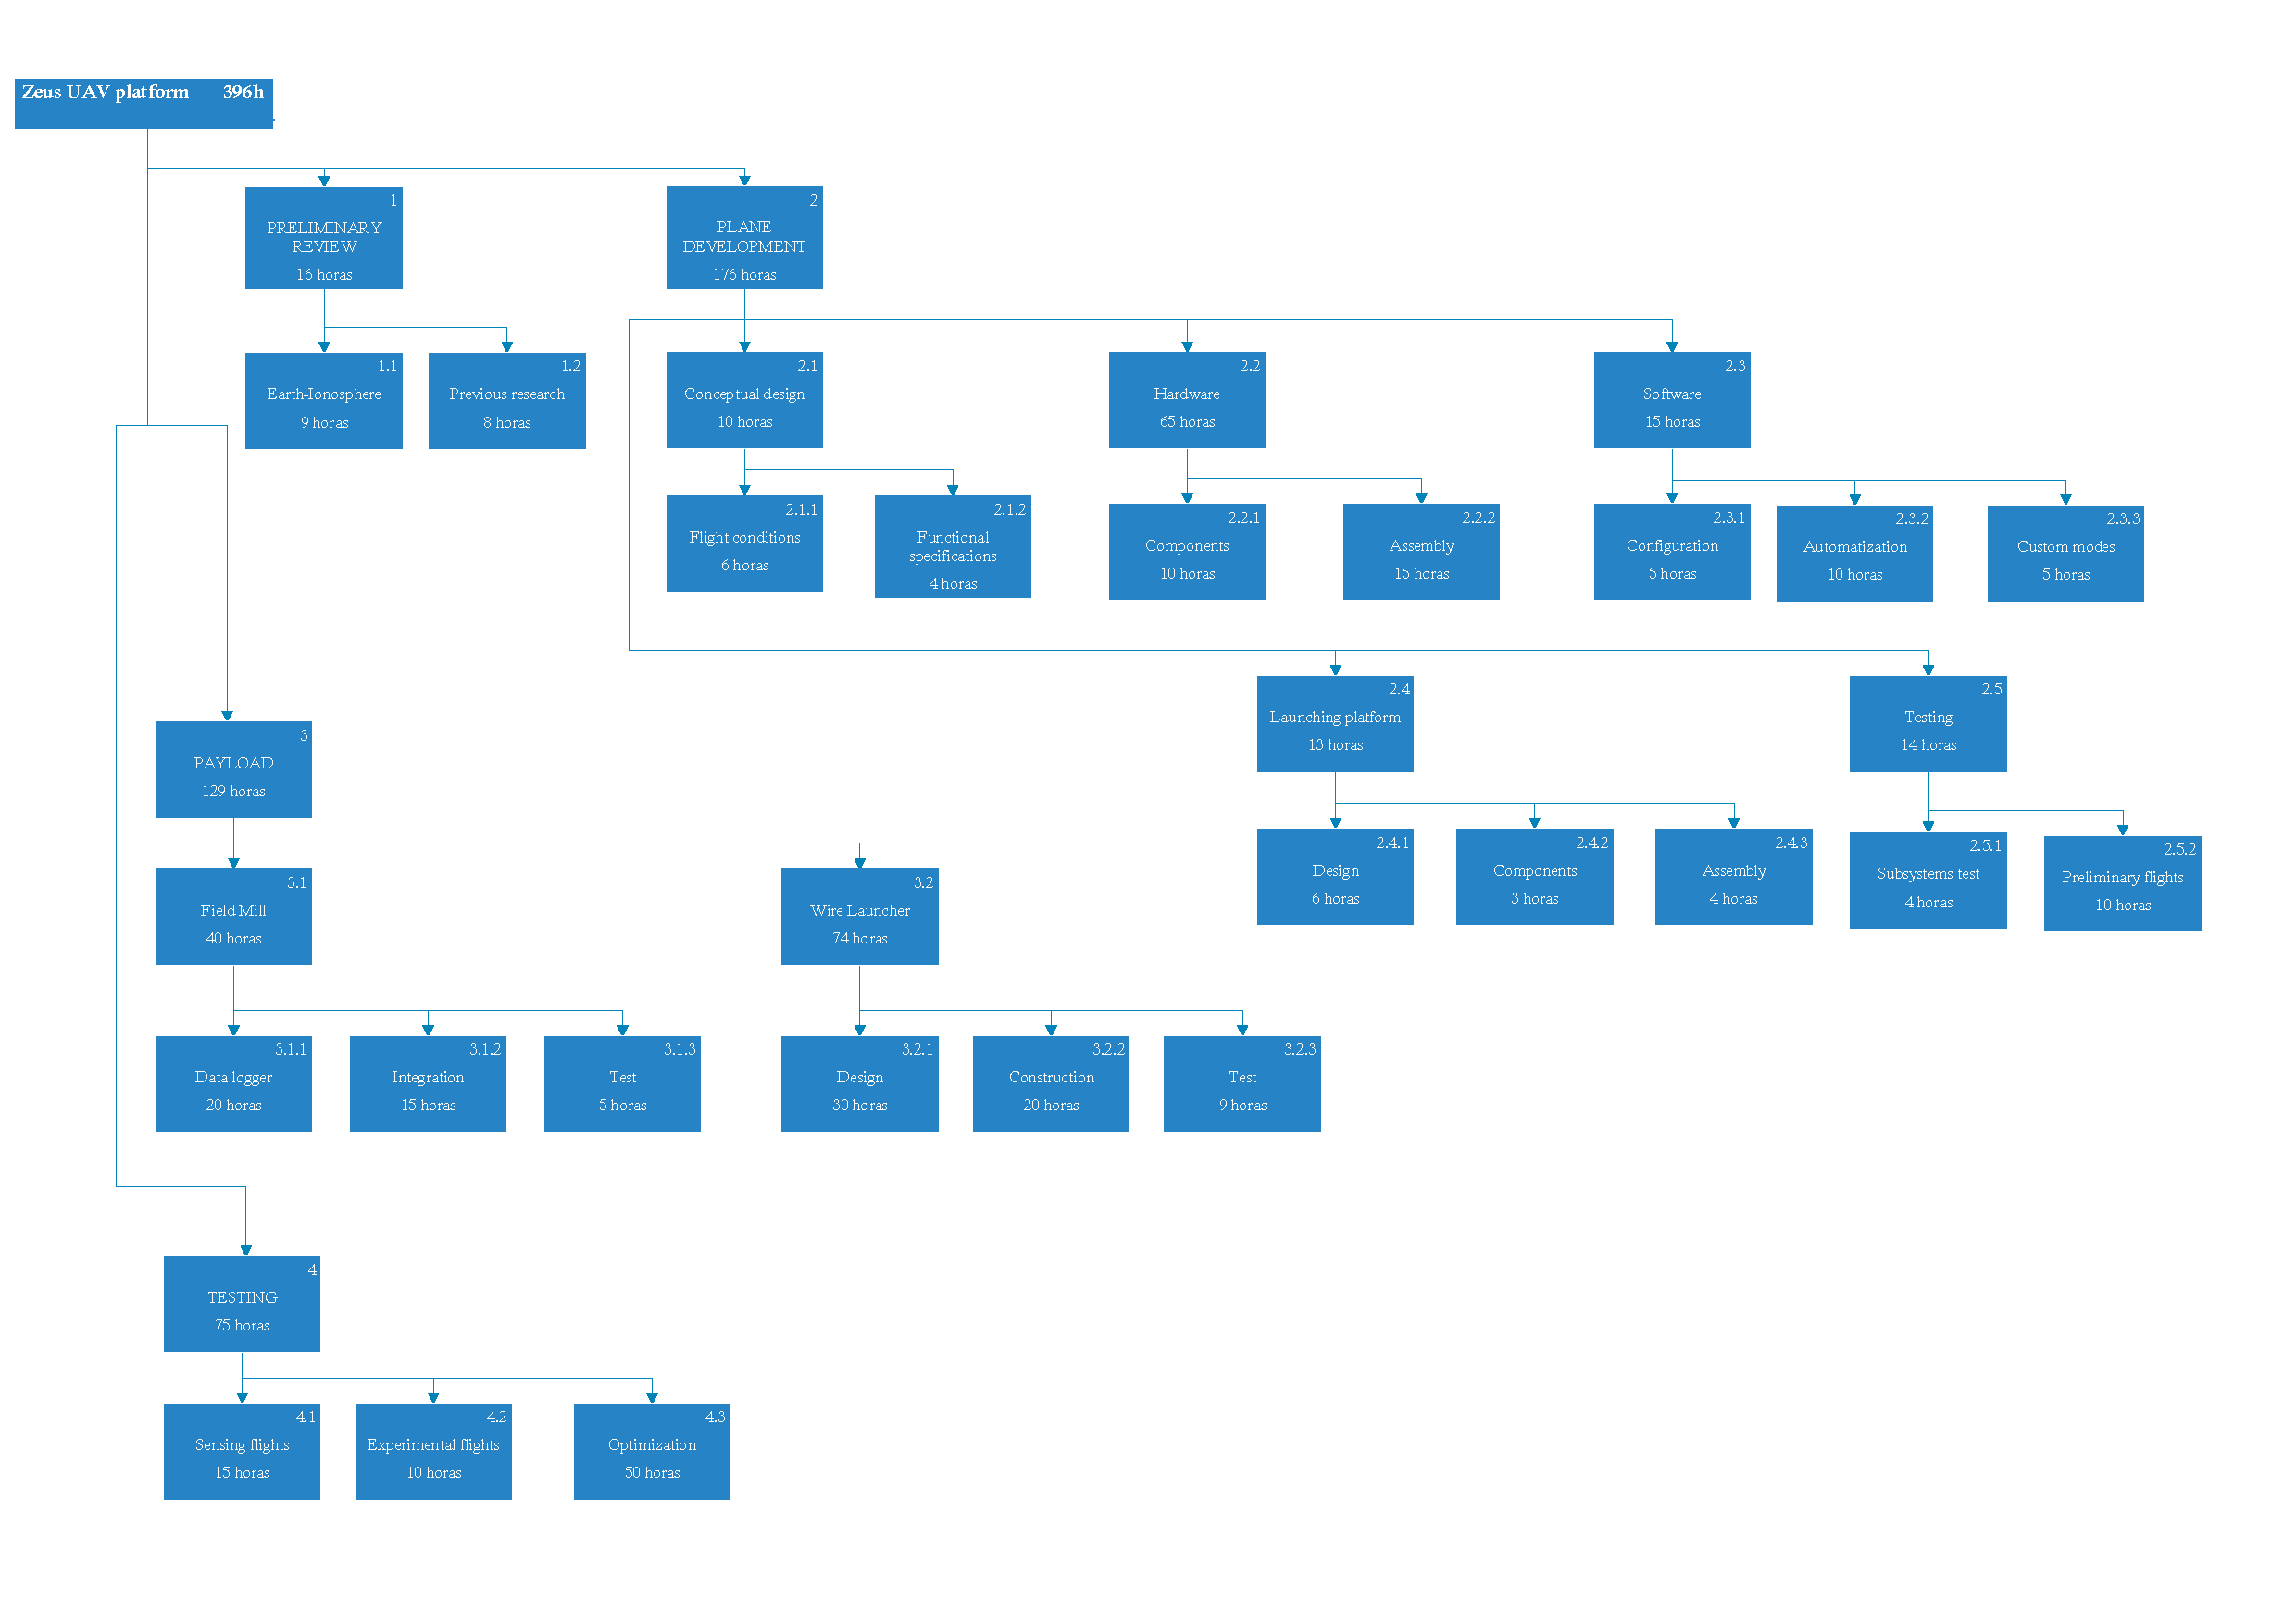
\includepdf{./pdf/WBS}

Si se quiere que la página también esté en horizontal, hay que utilizar \verb!\includepdf[landscape=true]{./pdf/nombre}!

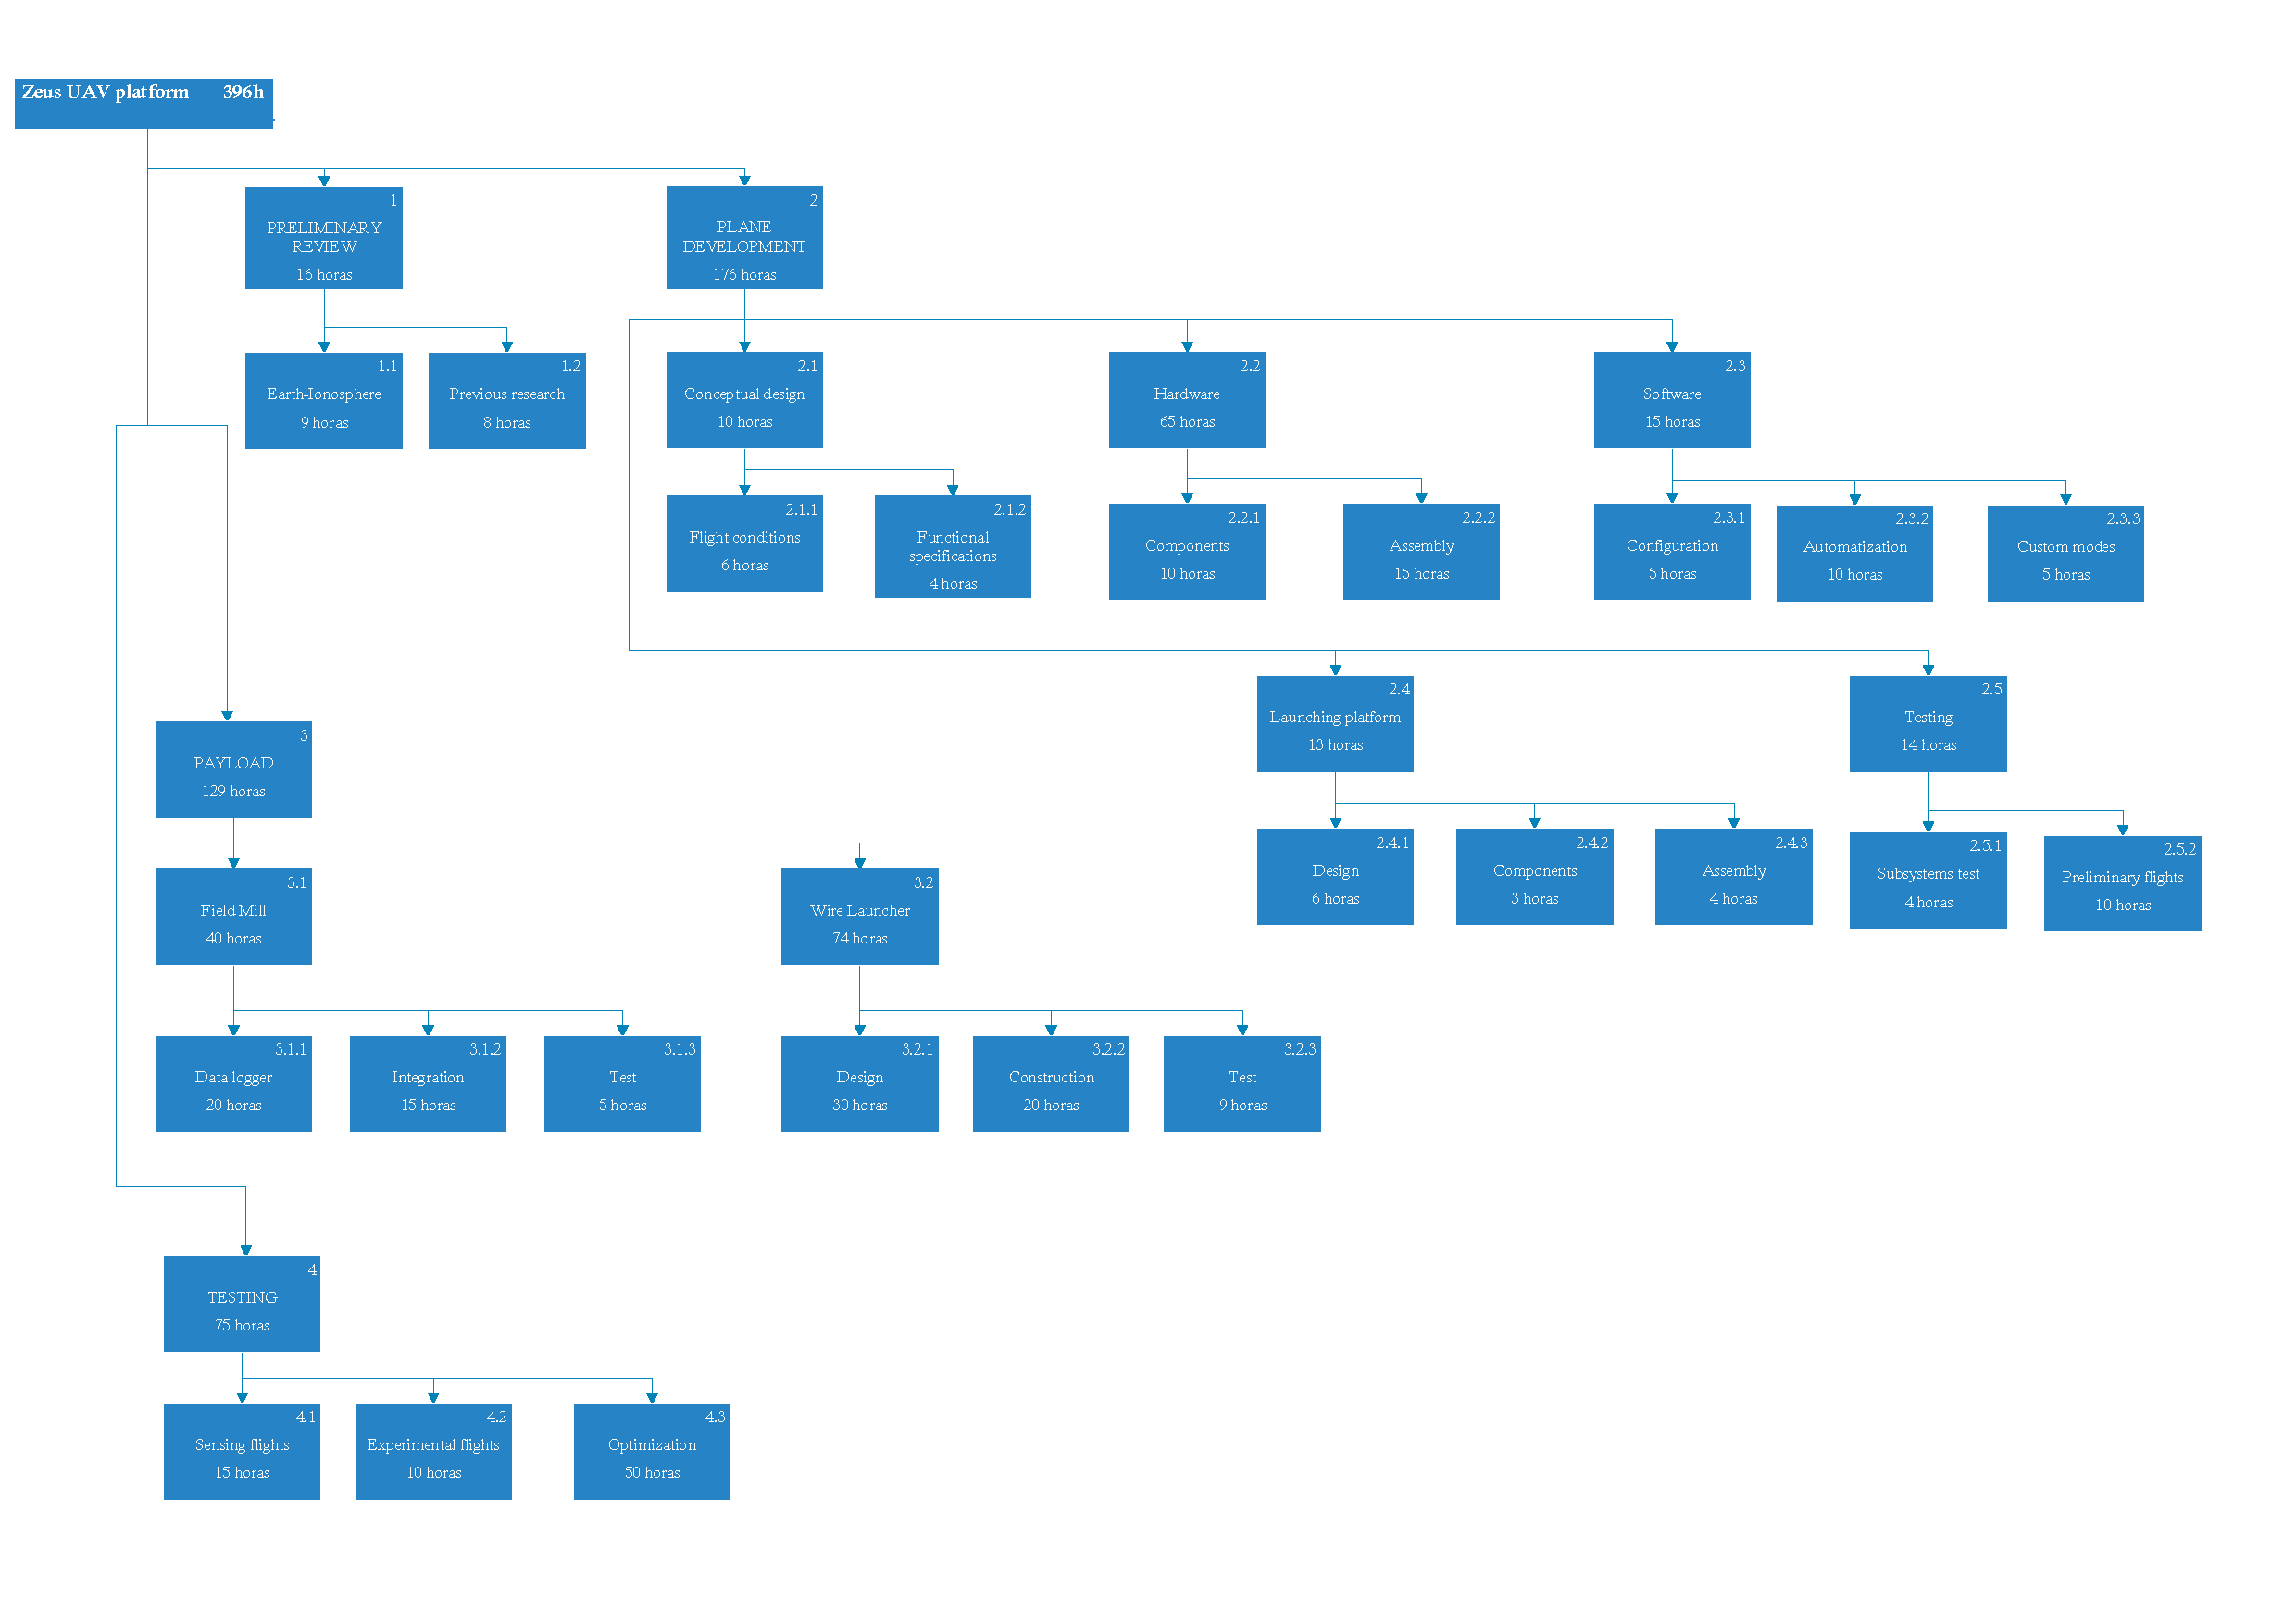
\includepdf[landscape=true]{./pdf/WBS}

Y para el número de páginas se aplica lo explicado anteriormente. Utilizando el comando \verb!\includepdf[landscape=true,pages=-]{./pdf/nombre}!, se insertan todas las páginas del pdf con la orientación de las páginas en horizontal

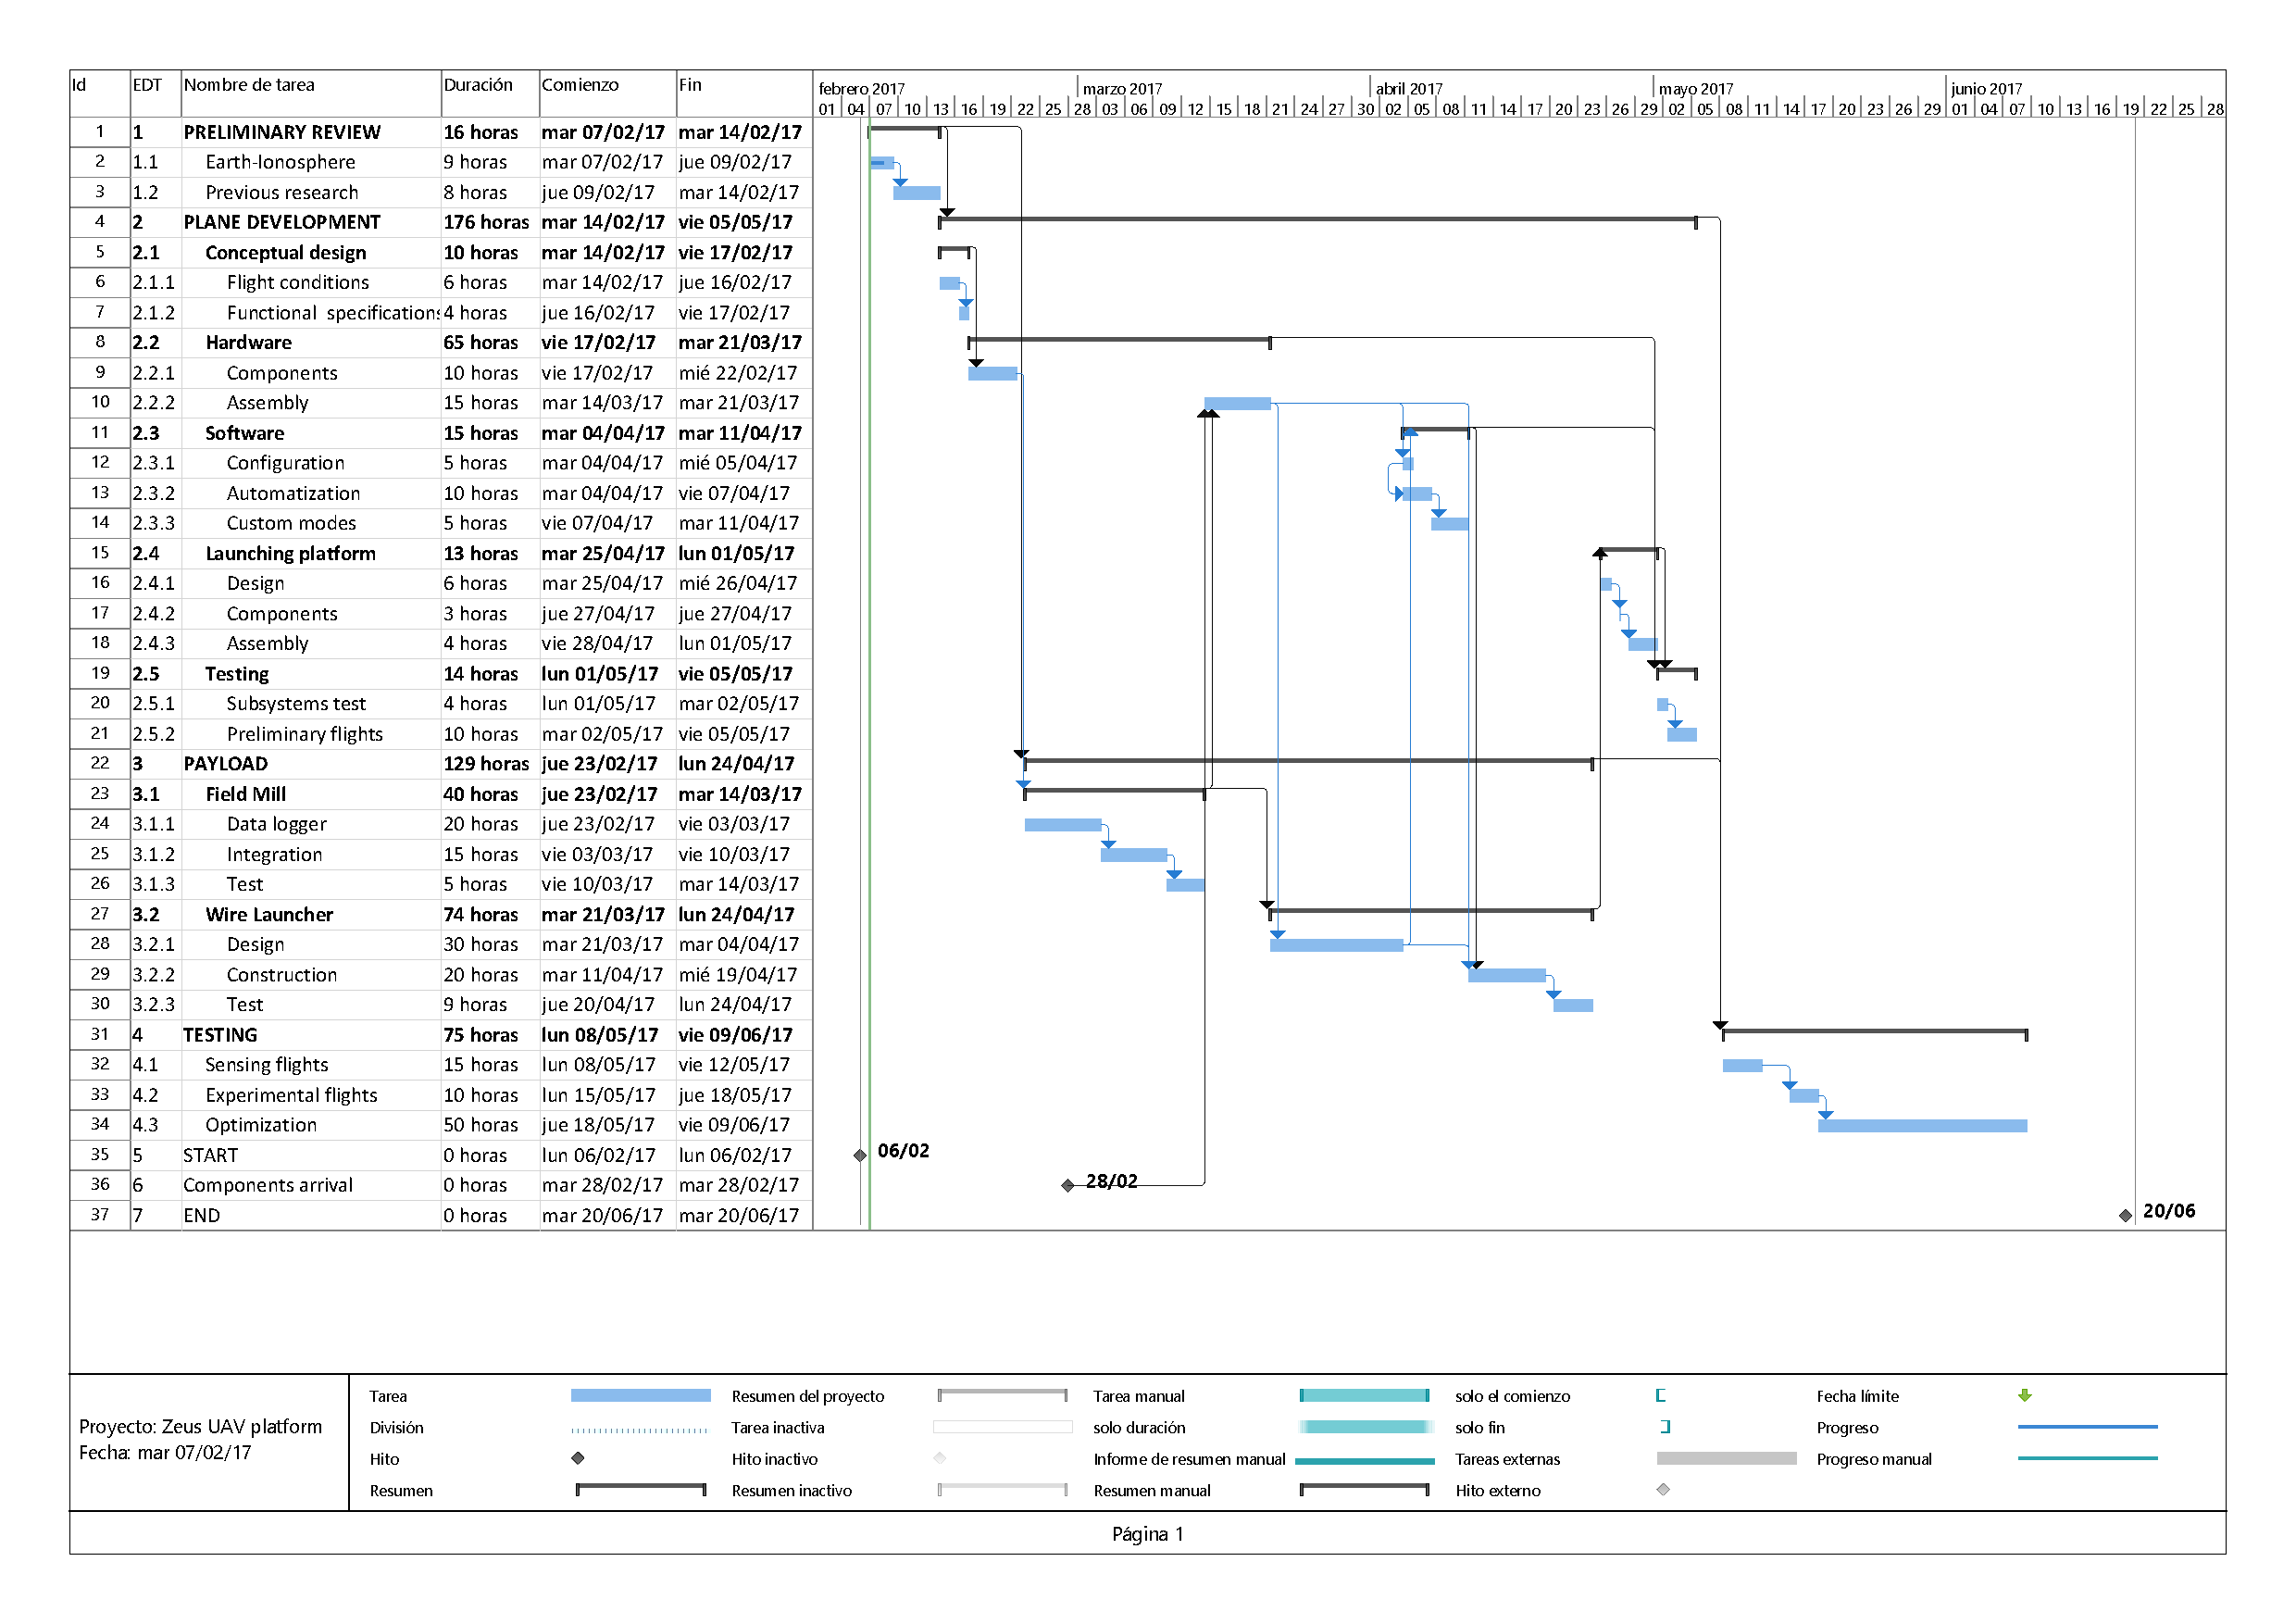
\includepdf[landscape=true,pages=-]{./pdf/GANTT}



% BIBLIOGRAPHY

% styles:
%	abbrv   : [#] Initial. Surname (pages and vol. abbrev.)
% 	acm     : [#] Surname, Initial. (sc)
%	alpha   : [Abrev.yy] Name Surname
%	apalike : [Surname, yyyy] Surname, Initial 
%	ieeetr  : [#] Initial. Surname (pages and vol. ext.)
%	plain   : [#] Name Surname
%	siam    : [#] Initial. Surname (sc)
%	unsrt   : [#] Name Surname

\bibliographystyle{plain}
\bibliography{bibliography} 


\end{document}